
\documentclass[
	11pt, % Set the default font size, options include: 8pt, 9pt, 10pt, 11pt, 12pt, 14pt, 17pt, 20pt
	%t, % Uncomment to vertically align all slide content to the top of the slide, rather than the default centered
	aspectratio=169, % Uncomment to set the aspect ratio to a 16:9 ratio which matches the aspect ratio of 1080p and 4K screens and projectors
]{beamer}


%import theme and packages

%beautiful equation setting
\usefonttheme[onlymath]{serif}
\AtBeginDocument{%
      \DeclareSymbolFont{pureletters}{T1}{lmr}{\mddefault}{it}%
      }
      
\graphicspath{{Images/}{./}} % Specifies where to look for included images (trailing slash required)

\usepackage{booktabs} % Allows the use of \toprule, \midrule and \bottomrule for better rules in tables
\usepackage{animate}
\usepackage{hyperref}
\hypersetup{
    colorlinks=true,
    linkcolor=blue,
    filecolor=magenta,      
    urlcolor=cyan,
    pdftitle={Overleaf Example},
    pdfpagemode=FullScreen,
    }
\usepackage{caption}
\setbeamertemplate{caption}
{\raggedright\insertcaption\par} 


\usepackage[style=verbose]{biblatex}
\addbibresource{ref.bib} 

%add algorthim package
\usepackage{bm}
\usepackage[ruled,longend,linesnumbered]{algorithm2e}
\usepackage{cleveref}
\renewcommand*{\algorithmcfname}{}
\renewcommand{\thealgocf}{Algorithm \ \arabic{algocf}}
%control the footnote fontsize
\renewcommand{\footnotesize}{\tiny}

% Add sources 
\usepackage[absolute,overlay]{textpos}

\setbeamercolor{framesource}{fg=gray}
\setbeamerfont{framesource}{size=\tiny}

\newcommand{\source}[1]{\begin{textblock*}{4cm}(8.7cm,8.6cm)
    \begin{beamercolorbox}[ht=0.5cm,right]{framesource}
        \usebeamerfont{framesource}\usebeamercolor[fg]{framesource} Source: {#1}
    \end{beamercolorbox}
\end{textblock*}}
%----------------------------------------------------------------------------------------
%	SELECT LAYOUT THEME
%----------------------------------------------------------------------------------------

% Beamer comes with a number of default layout themes which change the colors and layouts of slides. Below is a list of all themes available, uncomment each in turn to see what they look like.

%\usetheme{default}
%\usetheme{AnnArbor}
%\usetheme{Antibes}
%\usetheme{Bergen}
%\usetheme{Berkeley}
%\usetheme{Berlin}
%\usetheme{Boadilla}
%\usetheme{CambridgeUS}
%\usetheme{Copenhagen}
%\usetheme{Darmstadt}
%\usetheme{Dresden}
%\usetheme{Frankfurt}
%\usetheme{Goettingen}
%\usetheme{Hannover}
%\usetheme{Ilmenau}
%\usetheme{JuanLesPins}
%\usetheme{Luebeck}
\usetheme{Madrid}
%\usetheme{Malmoe}
%\usetheme{Marburg}
%\usetheme{Montpellier}
%\usetheme{PaloAlto}
%\usetheme{Pittsburgh}
%\usetheme{Rochester}
%\usetheme{Singapore}
%\usetheme{Szeged}
%\usetheme{Warsaw}

%----------------------------------------------------------------------------------------
%	SELECT COLOR THEME
%----------------------------------------------------------------------------------------

% Beamer comes with a number of color themes that can be applied to any layout theme to change its colors. Uncomment each of these in turn to see how they change the colors of your selected layout theme.

%\usecolortheme{albatross}
%\usecolortheme{beaver}
%\usecolortheme{beetle}
%\usecolortheme{crane}
%\usecolortheme{dolphin}
%\usecolortheme{dove}
%\usecolortheme{fly}
%\usecolortheme{lily}
%\usecolortheme{monarca}
%\usecolortheme{seagull}
%\usecolortheme{seahorse}
%\usecolortheme{spruce}
%\usecolortheme{whale}
%\usecolortheme{wolverine}

%----------------------------------------------------------------------------------------
%	SELECT FONT THEME & FONTS
%----------------------------------------------------------------------------------------

% Beamer comes with several font themes to easily change the fonts used in various parts of the presentation. Review the comments beside each one to decide if you would like to use it. Note that additional options can be specified for several of these font themes, consult the beamer documentation for more information.

\usefonttheme{default} % Typeset using the default sans serif font
%\usefonttheme{serif} % Typeset using the default serif font (make sure a sans font isn't being set as the default font if you use this option!)
%\usefonttheme{structurebold} % Typeset important structure text (titles, headlines, footlines, sidebar, etc) in bold
%\usefonttheme{structureitalicserif} % Typeset important structure text (titles, headlines, footlines, sidebar, etc) in italic serif
%\usefonttheme{structuresmallcapsserif} % Typeset important structure text (titles, headlines, footlines, sidebar, etc) in small caps serif

%------------------------------------------------

%\usepackage{mathptmx} % Use the Times font for serif text
\usepackage{palatino} % Use the Palatino font for serif text

%\usepackage{helvet} % Use the Helvetica font for sans serif text
\usepackage[default]{opensans} % Use the Open Sans font for sans serif text
%\usepackage[default]{FiraSans} % Use the Fira Sans font for sans serif text
%\usepackage[default]{lato} % Use the Lato font for sans serif text

%----------------------------------------------------------------------------------------
%	SELECT INNER THEME
%----------------------------------------------------------------------------------------

% Inner themes change the styling of internal slide elements, for example: bullet points, blocks, bibliography entries, title pages, theorems, etc. Uncomment each theme in turn to see what changes it makes to your presentation.

%\useinnertheme{default}
\useinnertheme{circles}
%\useinnertheme{rectangles}
%\useinnertheme{rounded}
%\useinnertheme{inmargin}

%----------------------------------------------------------------------------------------
%	SELECT OUTER THEME
%----------------------------------------------------------------------------------------

% Outer themes change the overall layout of slides, such as: header and footer lines, sidebars and slide titles. Uncomment each theme in turn to see what changes it makes to your presentation.

%\useoutertheme{default}
\useoutertheme{infolines}
%\useoutertheme{miniframes}
%\useoutertheme{smoothbars}
%\useoutertheme{sidebar}
%\useoutertheme{split}
%\useoutertheme{shadow}
%\useoutertheme{tree}
%\useoutertheme{smoothtree}

%\setbeamertemplate{footline} % Uncomment this line to remove the footer line in all slides
%\setbeamertemplate{footline}[page number] % Uncomment this line to replace the footer line in all slides with a simple slide count

%\setbeamertemplate{navigation symbols}{} % Uncomment this line to remove the navigation symbols from the bottom of all slides



%section name empty slides
\AtBeginSection[]{
  \begin{frame}
  \vfill
  \centering
  \begin{beamercolorbox}[sep=8pt,center,shadow=false,rounded=true]{title}
    \usebeamerfont{title}\insertsectionhead\par%
  \end{beamercolorbox}
  \vfill
  \end{frame}
}




%tikz packages

\usepackage{tikz}
\usepackage{adjustbox}


\usetikzlibrary{arrows.meta,
                chains, automata,
                positioning,
                shapes.geometric,
                %bayesnet,
                backgrounds,
                decorations.pathreplacing
                }

\newcommand{\edgex}[3][style={-latex}]{% edge with a new style <<<
	% Connect all nodes #2 to all nodes #3.
	\foreach \x in {#2} { %
		\foreach \y in {#3} { %
			\draw[#1,->] (\x) -- (\y) ;%
		} ;
	} ;
}
\tikzset{
  main/.style={circle, minimum size = 1.1cm, thick, draw =black!80, node distance = 10mm}
}



%%%%%%%%%%%%%%%%%%%%%%%%%%%%%%%%%%%%%%%%%%%%%%
%%%%%%%%%%%%%Appendix setting
\newcommand{\backupbegin}{
   \newcounter{finalframe}
   \setcounter{finalframe}{\value{framenumber}}
}
\newcommand{\backupend}{
   \setcounter{framenumber}{\value{finalframe}}
}



%import title page

%----------------------------------------------------------------------------------------
%	PRESENTATION INFORMATION
%----------------------------------------------------------------------------------------

\title[\textcolor{white}{UQ}]{Uncertainty quantification (UQ) in geotechnical engineering} % The short title in the optional parameter appears at the bottom of every slide, the full title in the main parameter is only on the title page

\subtitle{} % Presentation subtitle, remove this command if a subtitle isn't required

\author[Ningxin Yang]{Ningxin Yang} % Presenter name(s), the optional parameter can contain a shortened version to appear on the bottom of every slide, while the main parameter will appear on the title slide

\institute[IC]{Civil and Environmental Engineering, Imperial College London \\ \smallskip \textit{n.yang23@imperial.ac.uk}} % Your institution, the optional parameter can be used for the institution shorthand and will appear on the bottom of every slide after author names, while the required parameter is used on the title slide and can include your email address or additional information on separate lines

\date[\today]{\\ \today} % Presentation date or conference/meeting name, the optional parameter can contain a shortened version to appear on the bottom of every slide, while the required parameter value is output to the title slide
\titlegraphic{Supervisors: Dr Truong Le; Prof. Lidija Zdravković}

%----------------------------------------------------------------------------------------




%table of content 
\AtBeginSection[]
  {
    %\ifnum \value{framenumber}>0
      \begin{frame}<beamer>
      \frametitle{}
      \tableofcontents[currentsection]
      \end{frame}
    %\else
    %\fi
  }
  
\begin{document}

%----------------------------------------------------------------------------------------
%	TITLE SLIDE
%----------------------------------------------------------------------------------------

\begin{frame}
	\titlepage % Output the title slide, automatically created using the text entered in the PRESENTATION INFORMATION block above
\end{frame}

%----------------------------------------------------------------------------------------
%	TABLE OF CONTENTS SLIDE
%----------------------------------------------------------------------------------------

% The table of contents outputs the sections and subsections that appear in your presentation, specified with the standard \section and \subsection commands. You may either display all sections and subsections on one slide with \tableofcontents, or display each section at a time on subsequent slides with \tableofcontents[pausesections]. The latter is useful if you want to step through each section and mention what you will discuss.

\begin{frame}
	\frametitle{Presentation Overview} % Slide title, remove this command for no title
	
	\tableofcontents % Output the table of contents (all sections on one slide)
	%\tableofcontents[pausesections] % Output the table of contents (break sections up across separate slides)
\end{frame}

%----------------------------------------------------------------------------------------
%	PRESENTATION BODY SLIDES
%----------------------------------------------------------------------------------------

\section{\textcolor{black}{UQ and uncertainty types}} % Sections are added in order to organize your presentation into discrete blocks, all sections and subsections are automatically output to the table of contents as an overview of the talk but NOT output in the presentation as separate slides

%------------------------------------------------
\begin{frame}
\frametitle{What is Uncertainty Quantification (UQ)?}
\only<1>{\begin{quote}
    \Large All models are wrong, but some are useful.\\
    --George E.P. Box
\end{quote}
\bigskip

\hspace*{70pt} How inaccurate might the models be?\\
\hspace*{90pt}When are they useful in engineering problems?\\
\hspace*{110pt} How much confidence can we have in model's predictions?

\bigskip
\hspace*{130pt} \Large UQ provides a framework answering
\hspace*{140pt} these questions and making model useful.
}

\only<2>{
\begin{figure}
    \centering
    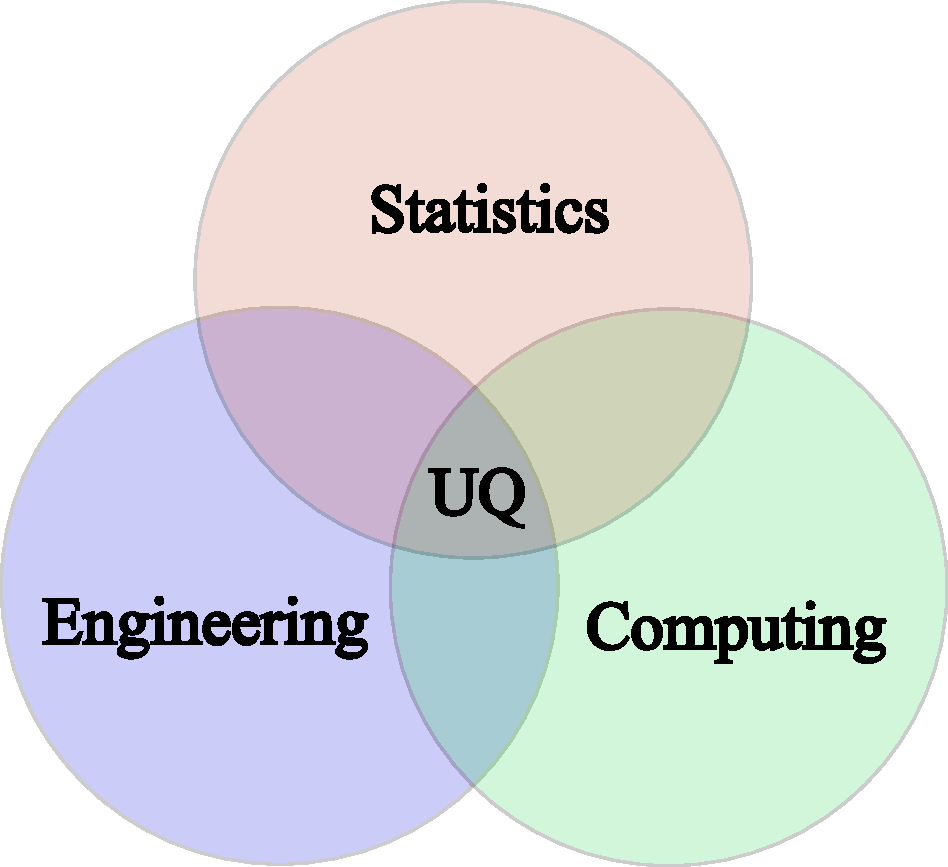
\includegraphics[width = 5.8cm]{figures/figure_UQ_subject.pdf}
    \label{fig:UQ-subject}
    \end{figure}

\begin{quote}
UQ is the science of quantitative \textcolor{red}{characterization} and \textcolor{red}{reduction} of uncertainties in both computational and real world applications\footfullcite{Saouma2021} 
\end{quote}
}



 \end{frame}
 %--------------------------------------------------------------------------------------------
 %-------------------------------------------------------------------

\begin{frame}
	\frametitle{Unforecast exposures in geotechnics}
    \begin{figure}
    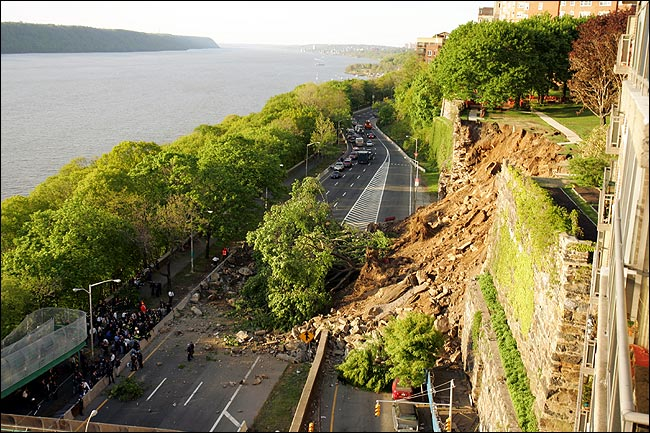
\includegraphics[height = 2.4cm]{figures/figure-geofailureone.jpg}    
    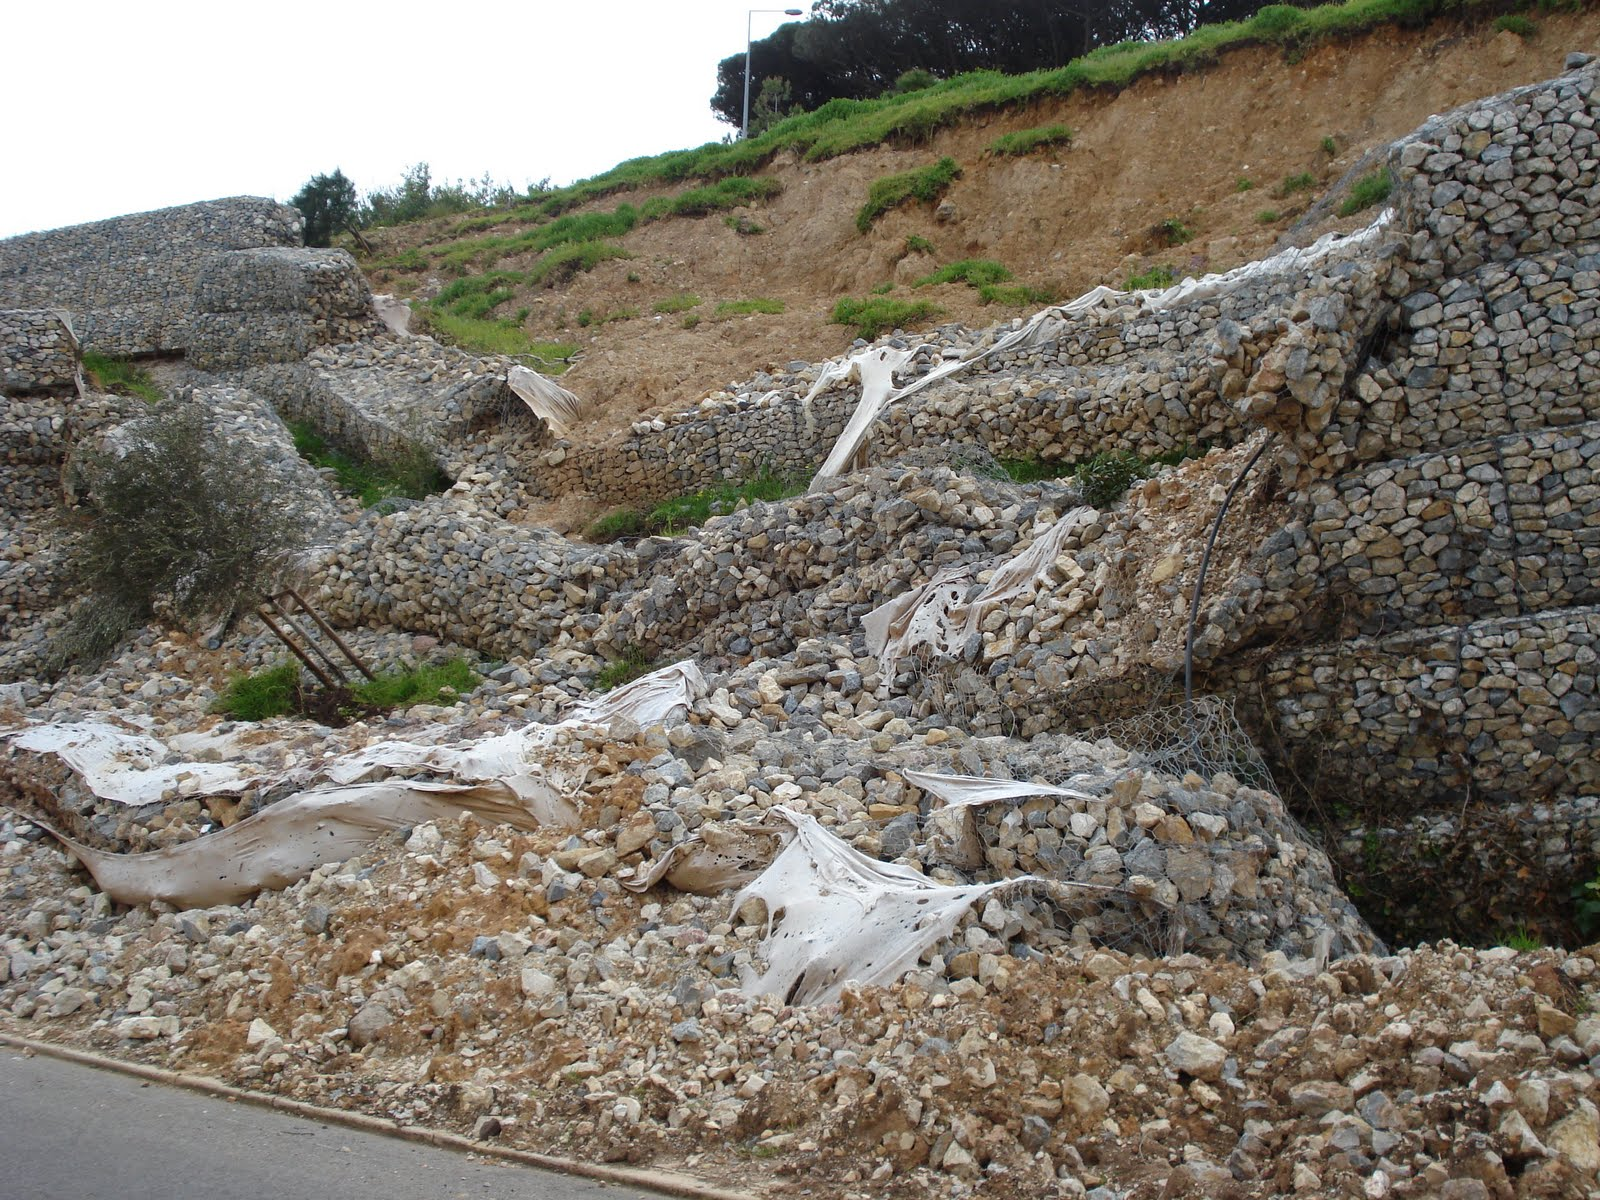
\includegraphics[height = 2.4cm]{figures/figure-geofailuretwo.jpg}  
    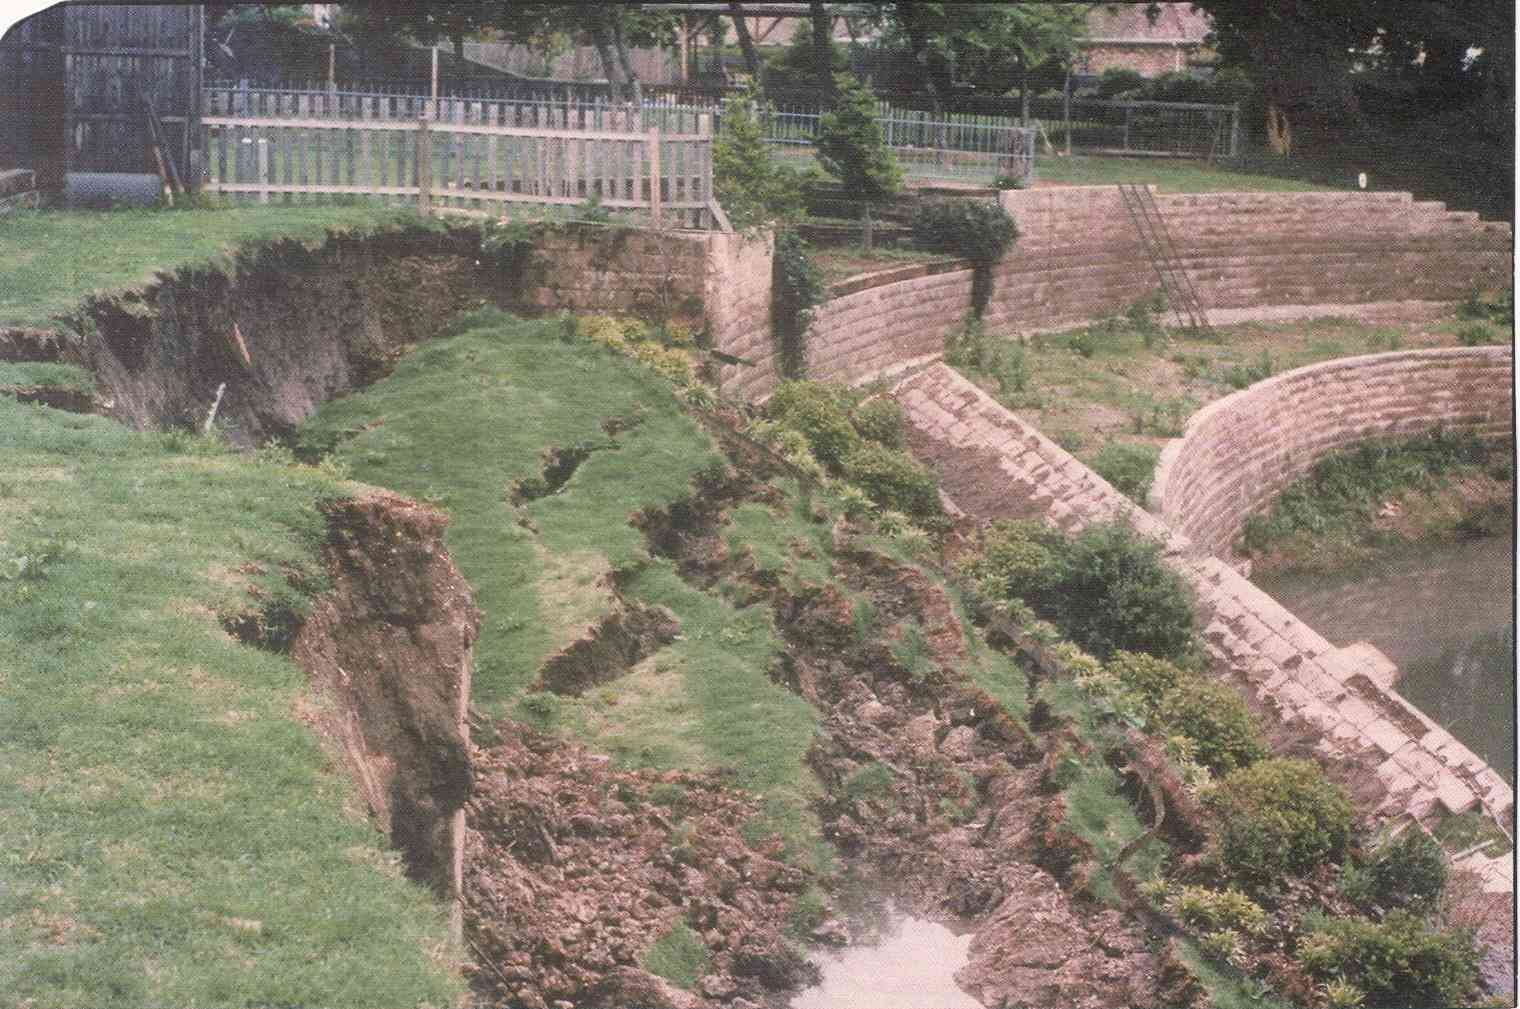
\includegraphics[height = 2.4cm]{figures/figure-geofailurethree.jpg}  
    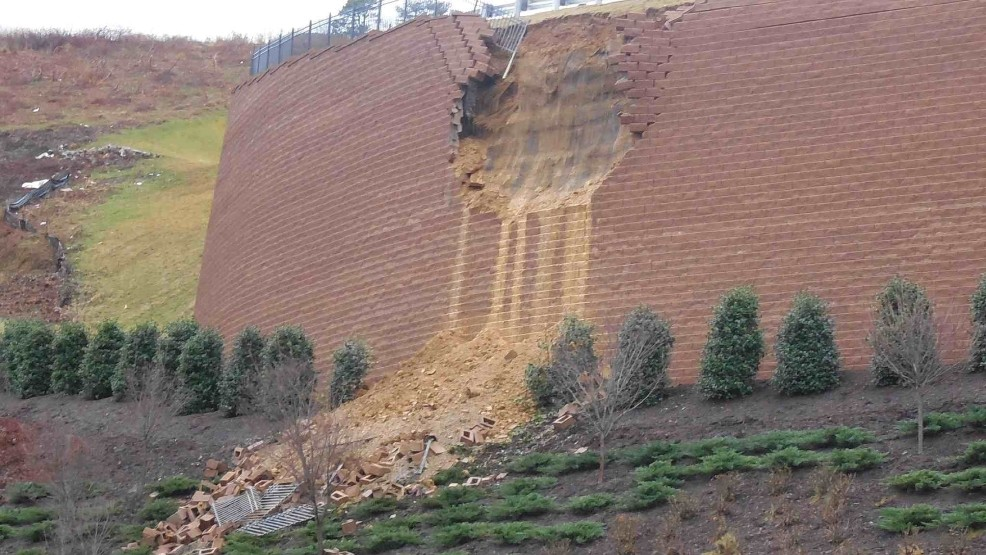
\includegraphics[height = 2.4cm]{figures/figure-geofailurefour.jpg}  
    \tiny\footnotetext{\href{https://www.capitalgeotechnical.com/geotechnical-failures.html}{capitalgeotechnical}}
    \end{figure}    
    
\end{frame}

%------------------------------------------------
\begin{frame}
\frametitle{Types of two uncertainties}
\framesubtitle{Aleatoric vs epistemic}

\begin{columns}
    \column{0.7\textwidth}
        \begin{figure}
        \centering
            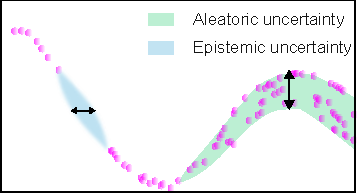
\includegraphics[width = 9cm]{figures/aleatoricvsepisidemic.pdf}
            \caption*{Aleatoric uncertainty vs Epistemic uncertainty}
        \end{figure} 
    \column{0.3\textwidth}
     \textbf{Distinguish}:
     \begin{block}{Aleatoric uncertainty}
statistical variability, inherently random effects (\textbf{irreducible})
     \end{block}
     \begin{block}{Epistemic uncertainty}
model uncertainty, a lack of knowledge (\textbf{reducible})
     \end{block}    
    \end{columns}
\end{frame}
%--------------------------------
\begin{frame}
\frametitle{Uncertainty components:}
\Large\textbf{Total uncertainty $\approx$ aleatoric uncertainty $+$ epistemic uncertainty}
\begin{figure}
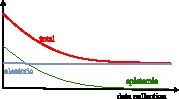
\includegraphics[scale=2.5]{figures/figure-total_Uncertainty.pdf}
\end{figure}

\end{frame}
%----------------------------------------------------------
\begin{frame}
\frametitle{Not simple as it is}
\framesubtitle{Mix of aleatoric and epistemic: Involve too much subjectivity}
\begin{figure}
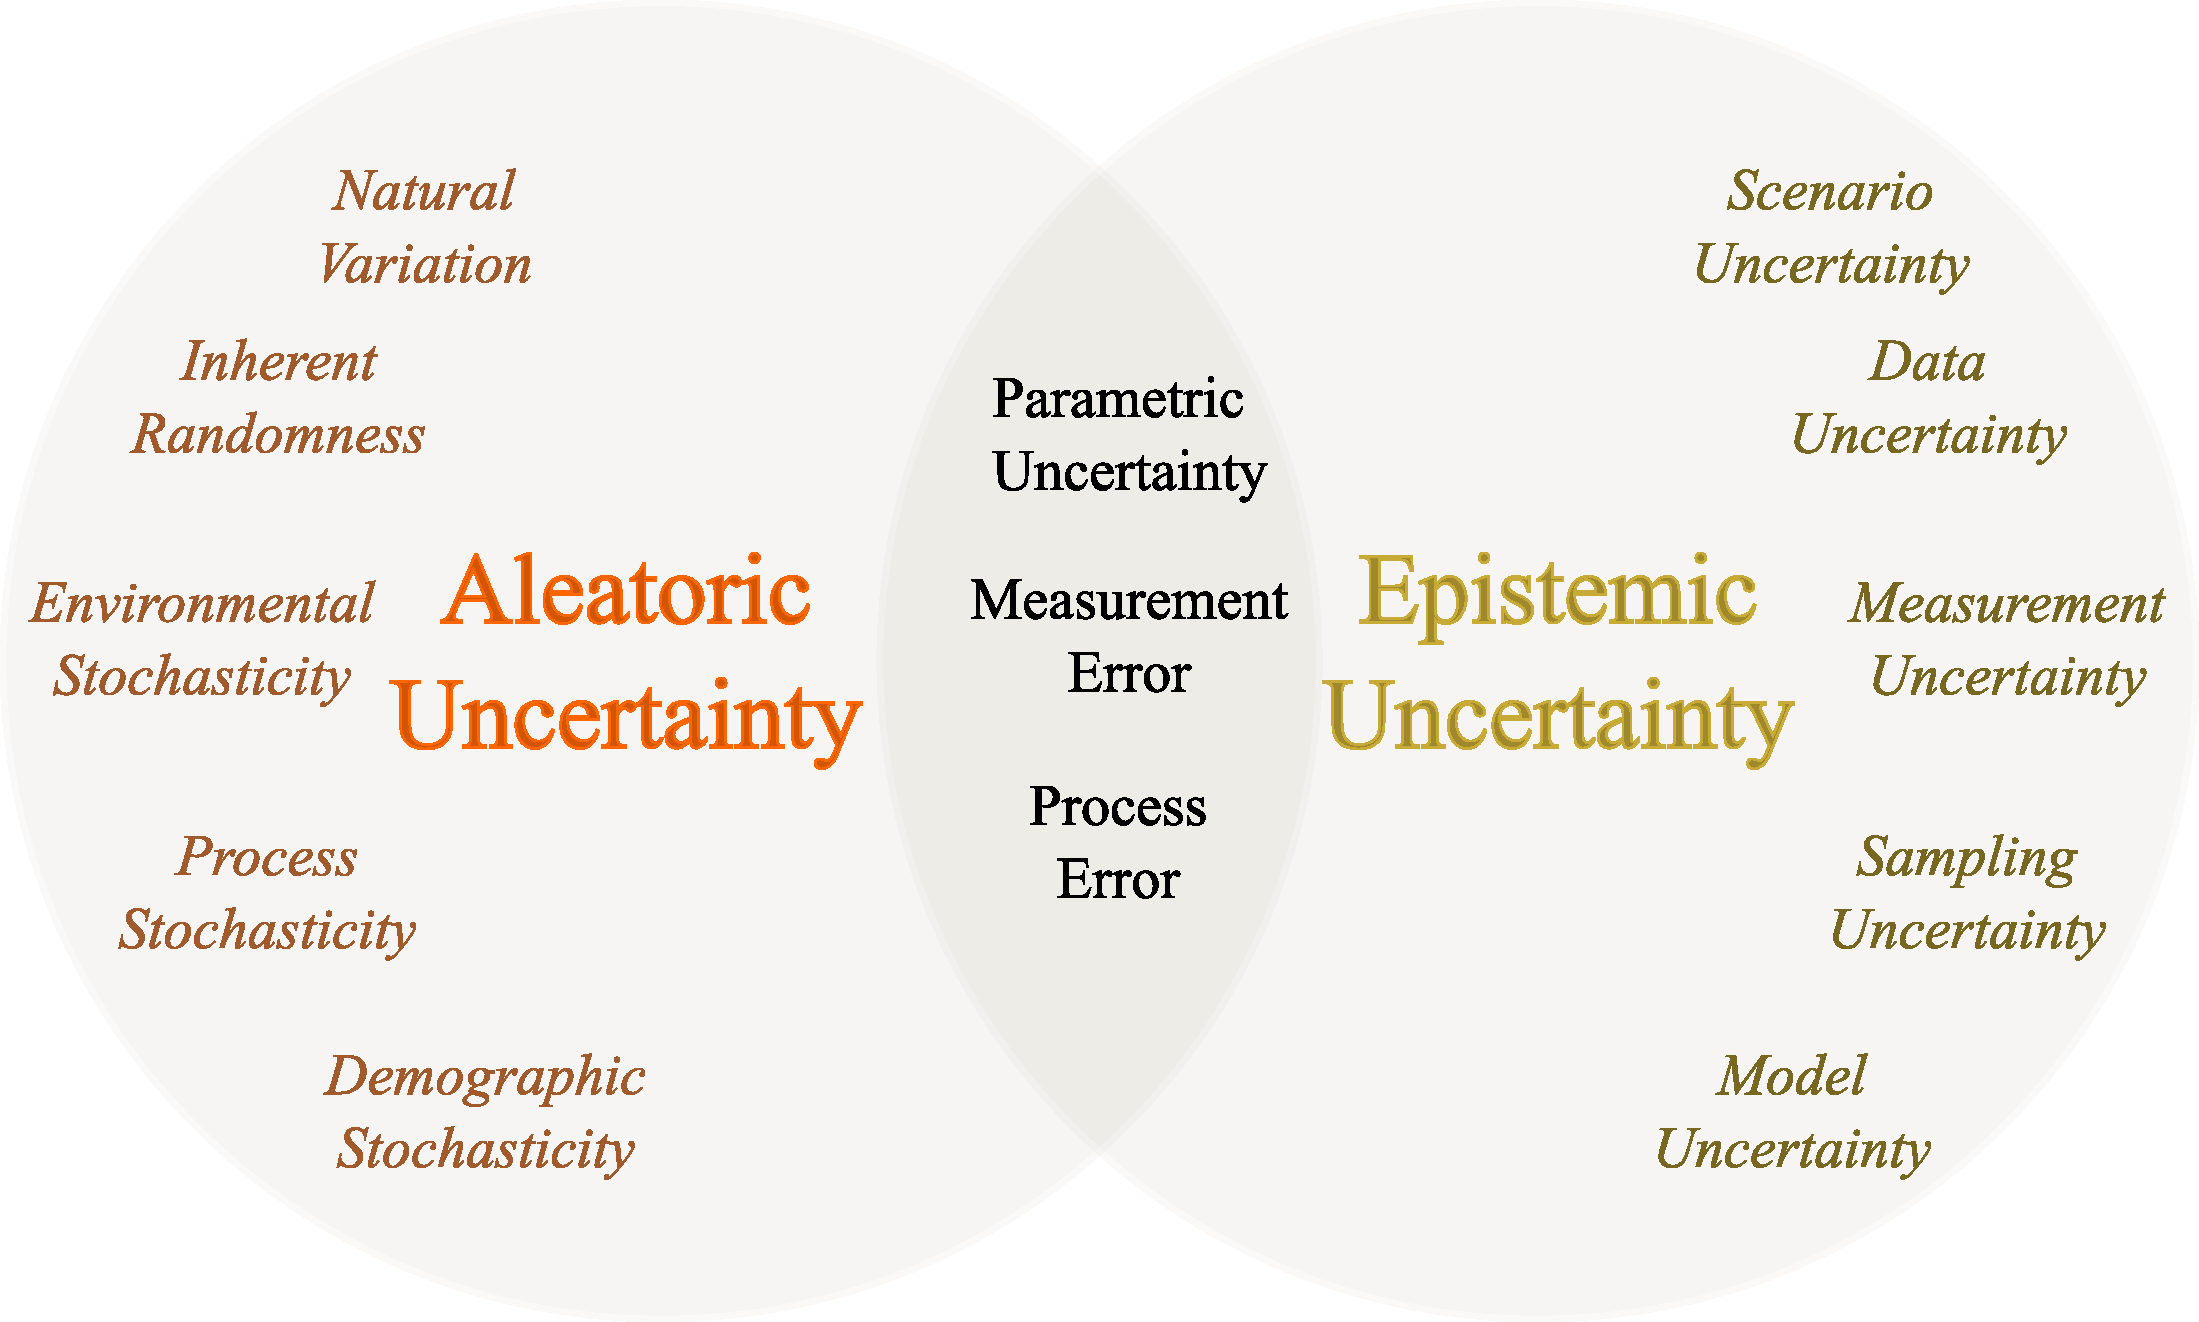
\includegraphics[scale=0.3]{figures/figure-uncertainty_classification.pdf}
\end{figure}
\end{frame}

%----------------------------------------------------------------------------
\begin{frame}
\frametitle{Examples in geotechnics}
    \begin{figure}
    \centering
    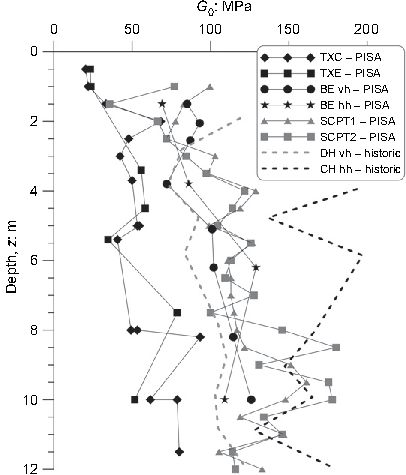
\includegraphics[scale=0.7]{figures/figure-UQtype2.pdf}
    \tiny\footcite{zdravkovic2020}
    \hspace{1cm}
    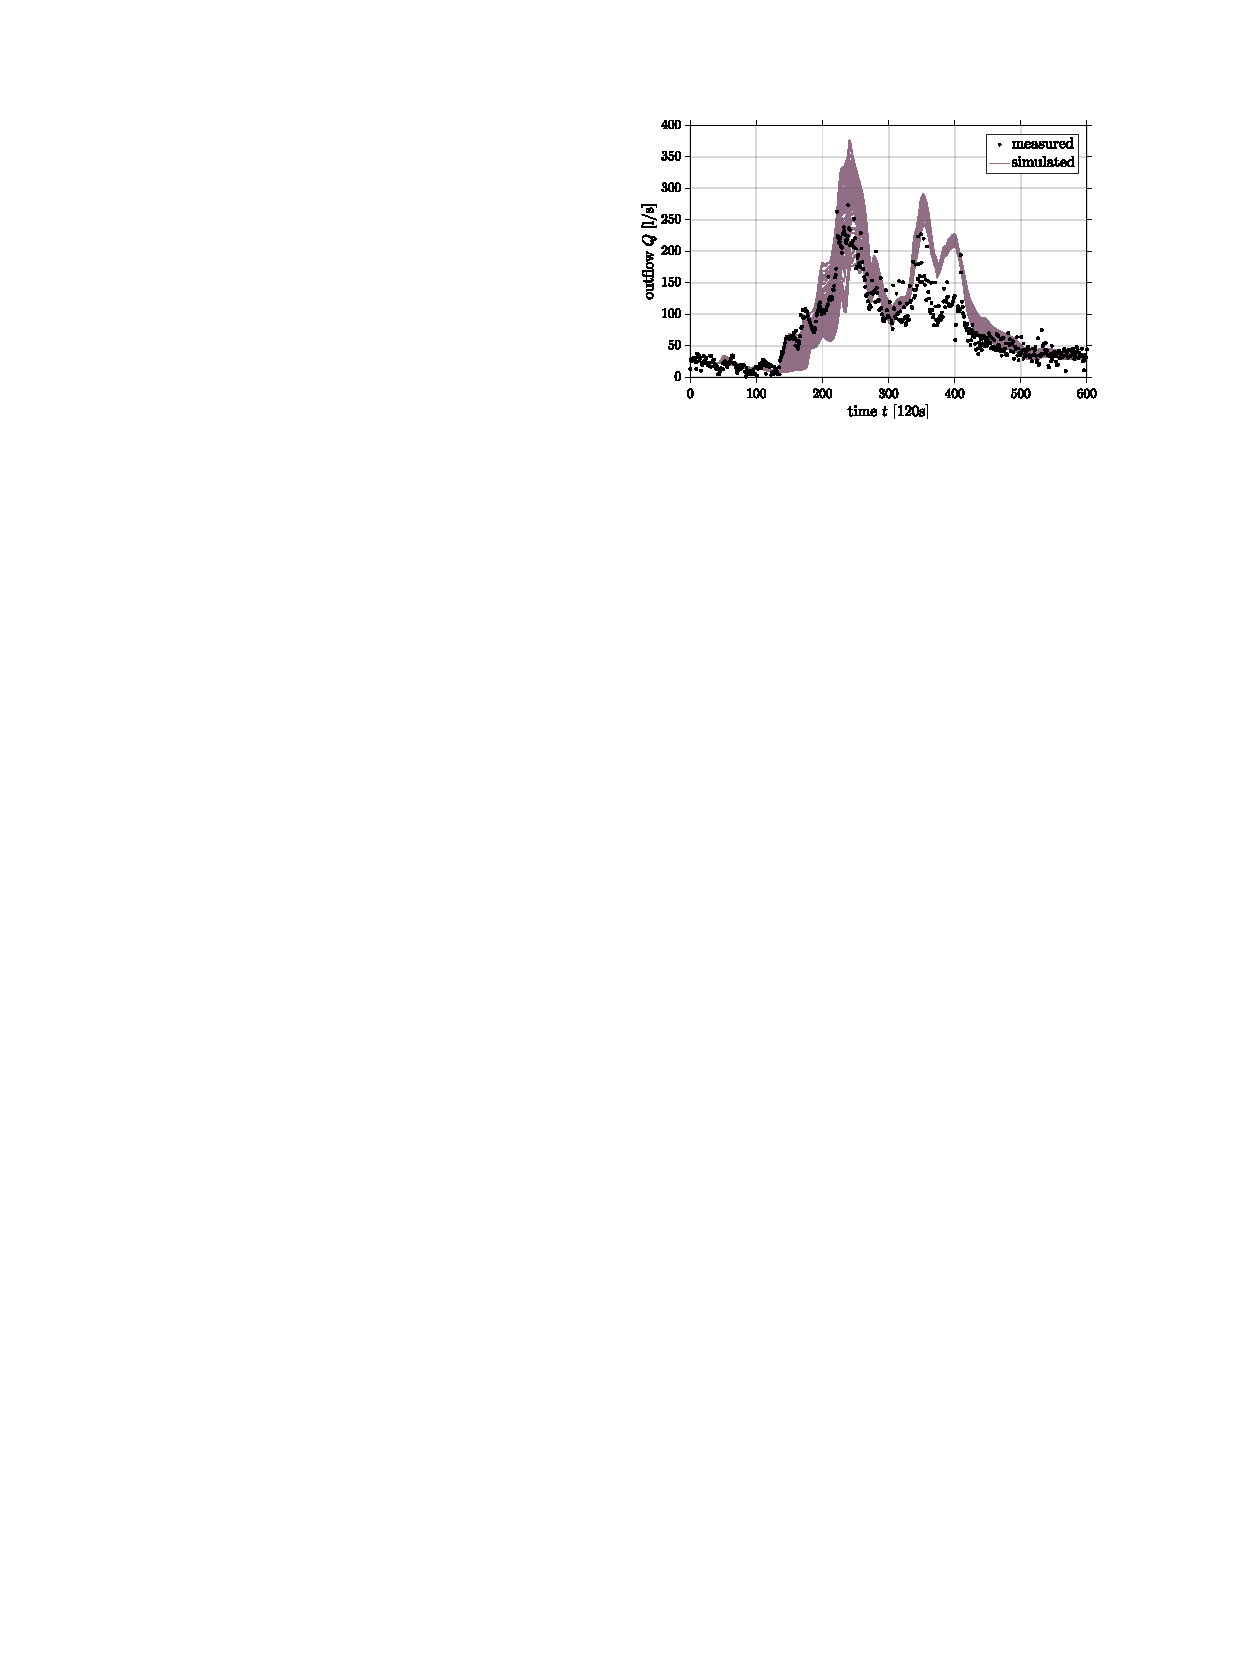
\includegraphics[scale=0.8]{figures/figure-UQtype3.pdf}
    \tiny\footcite{nagel2020}  
    \end{figure}
\end{frame}


\section{\textcolor{black}{UQ framework and components}}
%------------------------------------------------
\begin{frame}
\frametitle{Experiments, Models, Simulations, and UQ}
\begin{figure}
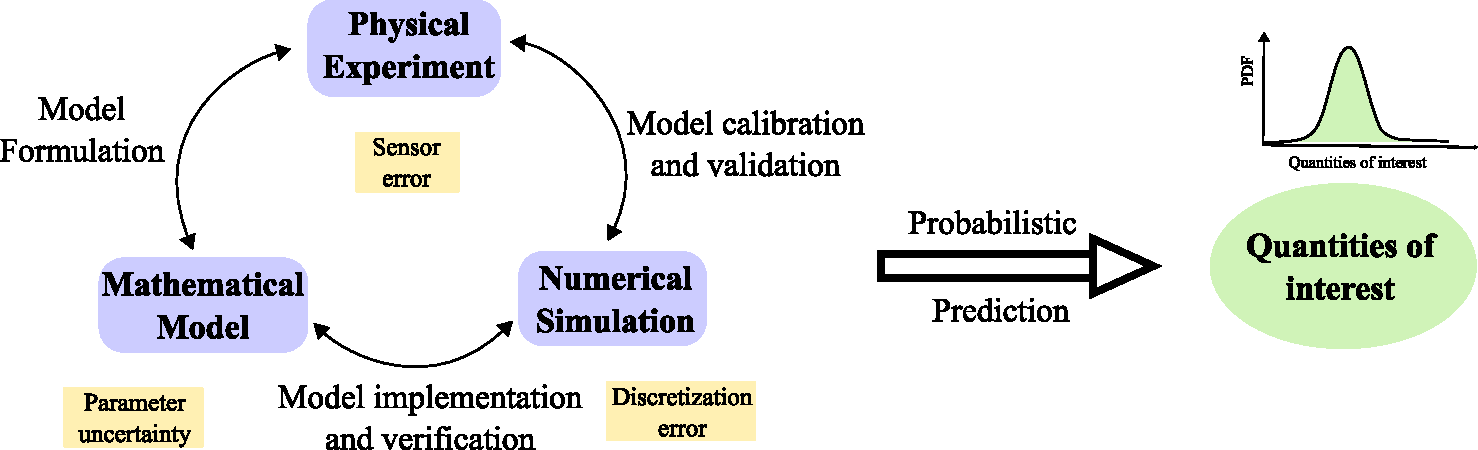
\includegraphics[scale=0.6]{figures/figure-UQ_physics_Model_Simulation.pdf}
\end{figure}
\end{frame}

%------------------------------------------------
\begin{frame}
\textbf{\frametitle{UQ problems and components}
\only<1>{
\begin{figure}
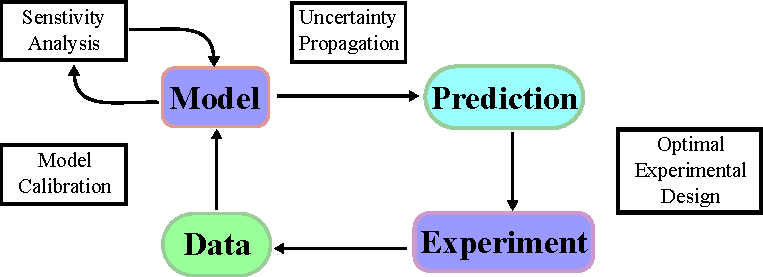
\includegraphics[scale=0.9]{figures/figure-UQ_components.pdf}
\end{figure}}
}
\only<2>{
\begin{block}{Two UQ types of problems:}
  \begin{figure}
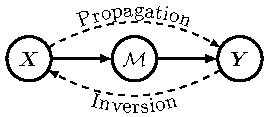
\includegraphics[width=6.5cm]{figures/figure_UQ_propagation_inversion.pdf}
\end{figure}  
\end{block}
\begin{block}{Four components:}
\begin{enumerate}
    \item Uncertainty propagation
    \item Model calibration
    \item Sensitivity analysis
    \item Optimal experimental design
\end{enumerate}  
\end{block}

}

\end{frame}

%------------------------------------------------
\begin{frame}
\framesubtitle{} % Optional subtitle
\begin{definition}
  A computational model should contain:
    \begin{itemize}
        \item a \alert{mathematical description} of the physics 
        \item may be seen as a \alert{black box} to compute the QoI
    \end{itemize}
\end{definition}
\only<1>{
        \begin{figure}            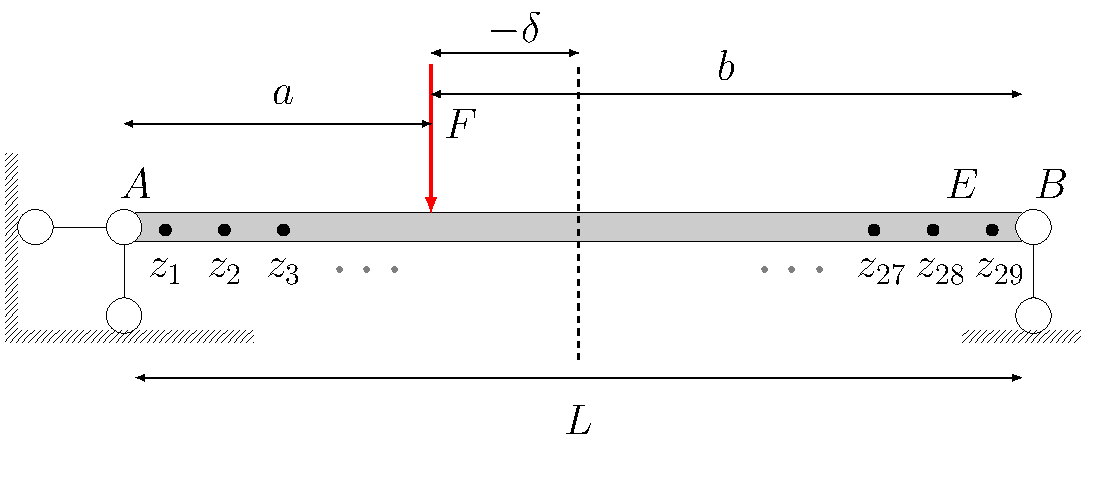
\includegraphics[scale=0.4]{figures/figure-beam.pdf}
        \end{figure}          
        \begin{equation}
                    y = \left\{\begin{matrix}
        \frac{F b  x  [(L^2 - b^2) - x^2]}{6LEI}  \ x \le a
         \\
         \frac{F b  [\frac{L}{b} (x - a)^3 + (L^2 - b^2)]}{6LEI} \ x> a
        \end{matrix}\right.
        \end{equation}
        }
        
\only<2>{
\begin{figure}
    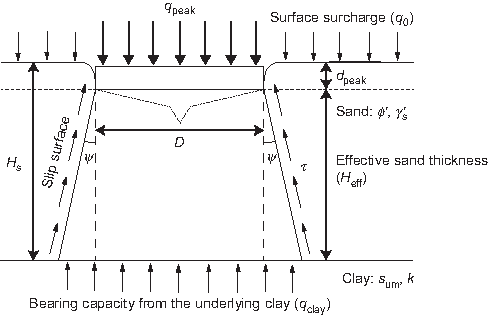
\includegraphics[scale=0.8]{figures/figure-qpeak.pdf}\footfullcite{li2018}
\end{figure}
}

\only<3>{
\bigskip
Numerical methods:
\begin{itemize}
    \item Finite element method
    \item Finite difference method
    \item $\cdots$
\end{itemize}
}
\end{frame}

%------------------------------------------------------------------------------------------------------------------------




%-----------------------------------------------------------------------------------------------------------------------
\begin{frame}
 \frametitle{UQ components one-Uncertainty propagation}
 \only<1>{
 \begin{figure}
    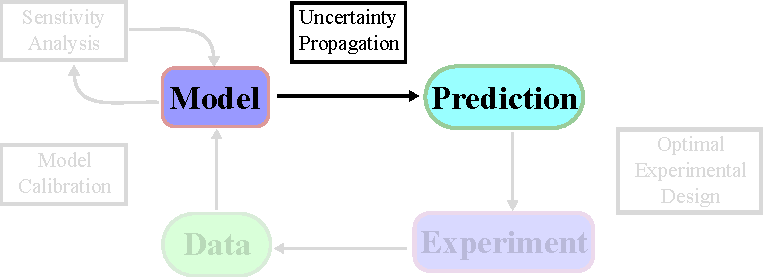
\includegraphics[scale=0.9]{figures/figure-UQcomponetone-propagation.pdf}
\end{figure}
\begin{itemize}
    \item \alert{Uncertainty propagation} feeds quantified input uncertainties through our model to produce probabilistic predictions of a QoI
\end{itemize}
 }

 \only<2>{
 \begin{figure}
    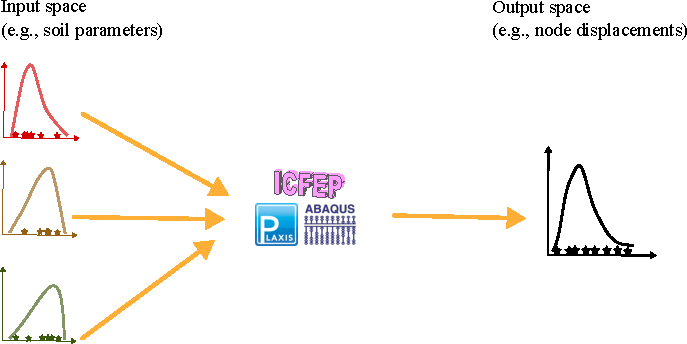
\includegraphics[scale=0.9]{figures/figure-UQ_propagation_MC.pdf}
\end{figure}
\begin{itemize}
\setlength\itemsep{0.5cm}
\item \alert{Output statistics}, i.e., mean, standard deviation. etc.
\begin{equation*}
    \mu_{\boldsymbol{Y}} = \mathbb{E}_{\boldsymbol{X}}
[\mathcal{M}(\boldsymbol{X}) ]; \ 
\sigma^2_{\boldsymbol{Y}} = \mathbb{E}_{\boldsymbol{X}}
[(\mathcal{M}(\boldsymbol{X}) - \mu_{\boldsymbol{Y}})^2]
\end{equation*}
\item \alert{Distribution} of the QoI
\item \alert{Probability} of exceeding an admissible threshold $y_{adm}$ following $P_{f} = \mathbb{P}(\boldsymbol{Y} \ge y_{adm})$
\end{itemize}
 }



 \end{frame}

 %---------------------------------------------------------------------------------------------------
\begin{frame}
 \frametitle{UQ components two-Model calibration}
 \only<1>{
 \begin{figure}
    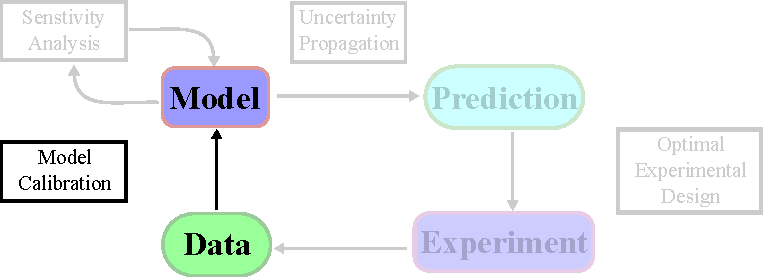
\includegraphics[scale=0.9]{figures/figure-UQcomponetwo-calibration.pdf}
\begin{itemize}
    \item \alert{Model calibration} explicitly quantifies model input uncertainties using experimental data (improve/update initial assumptions)
\end{itemize}
\end{figure}
 }

 \only<2>{
 \framesubtitle{Choice for UQ inversion}
\begin{columns}
    \column{0.5\textwidth}
        Choice for the UQ method is totally based on the {\textcolor{red}{\textbf{quantity}}} of accessible data:
        \begin{itemize}
            \item  {\textcolor{red}{\textbf{Lack}}} or {\textcolor{red}{\textbf{no}}} data available, model can be solely based on expert judgement
            \item {\textcolor{red}{\textbf{Substantial}}} volume data available, model can fully use statistical inference (e.g., the methods of moments)
            \item {\textcolor{red}{\textbf{Combination}}} of two above: Bayesian methods
            \begin{equation*}           \pi(\boldsymbol{x}|\mathcal{Y}) = \frac{{\mathcal{L}(\boldsymbol{x}|\mathcal{Y}) \cdot \pi(\boldsymbol{x})}}{{\pi(\mathcal{Y})}} 
            \end{equation*}
        \end{itemize}
    
    \column{0.5\textwidth}
        \begin{figure}[!ht]      
        %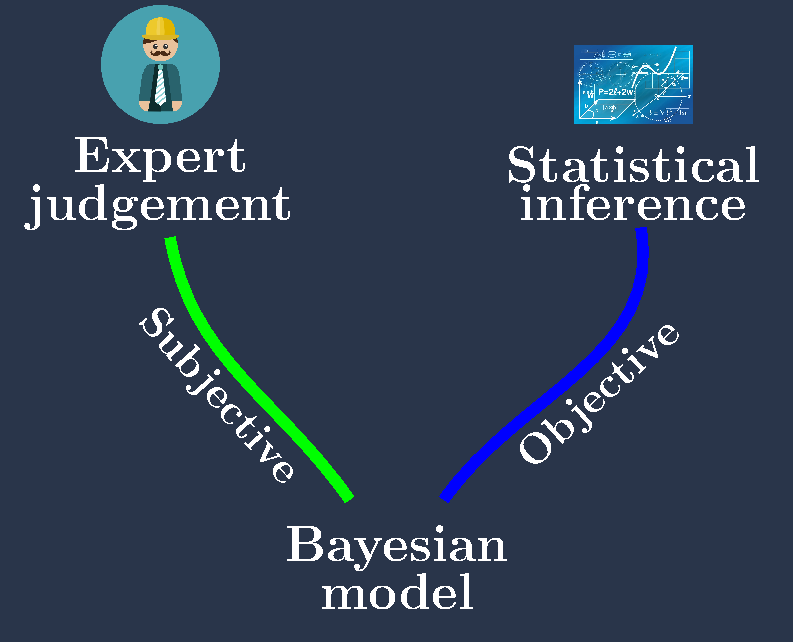
\includegraphics[scale=0.6]{figures/figure_objvssub.pdf}
        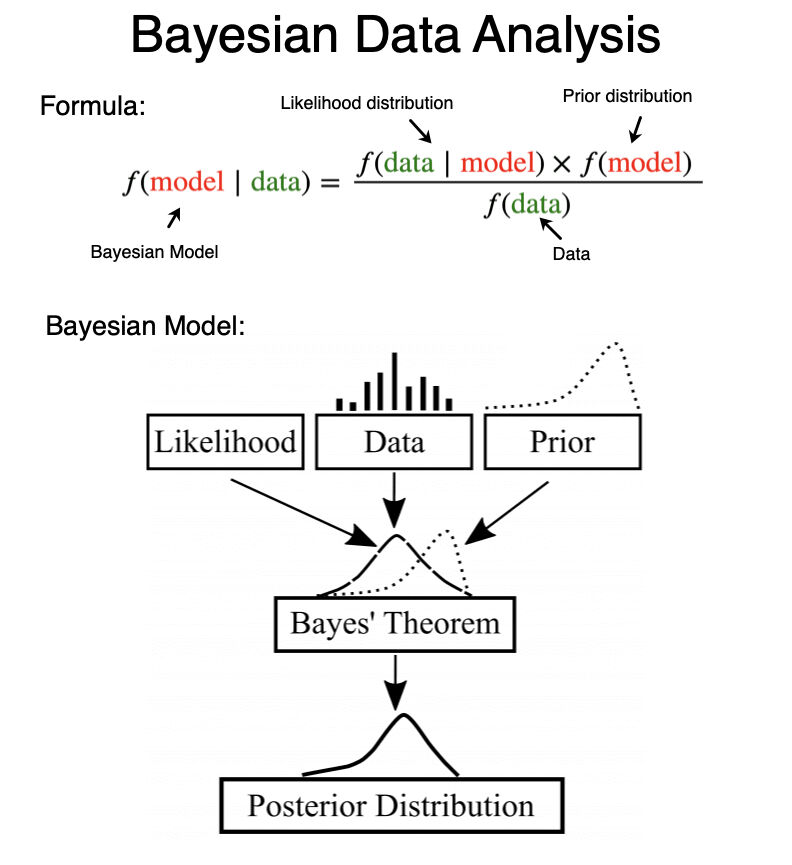
\includegraphics[scale=0.22]{figures/figure_Bayesflow.jpg}
        \end{figure}
\end{columns}
 }


\only<3>{
\begin{block}{Bayesian methods}
    Expert guess + Limited data $\rightarrow$ Distribution
\end{block}
\begin{columns}
    \column{0.5\textwidth}
    Prior:
    \begin{figure}[!ht]       
    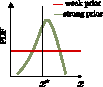
\includegraphics[scale=2]{figures/figure-weakandstrongprior.pdf}
    \end{figure}
    
    \column{0.5\textwidth}
    Likelihood:
    \begin{figure}[!ht]       
    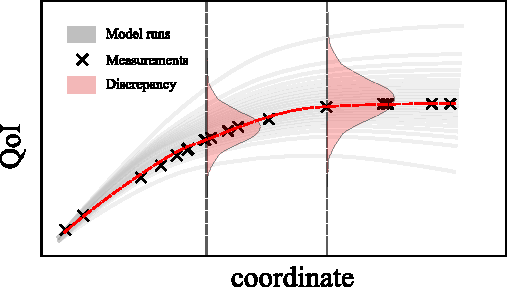
\includegraphics[scale=0.6]{figures/figure-likelihood.pdf}
    \end{figure} 
\end{columns}
\begin{alertblock}{Notable caveats:}
\begin{itemize}
    \item Prior-Requires specific expertise
    \item Likelihood-Computationally expensive 
\end{itemize}  
\end{alertblock}
}



 \end{frame}
 %======================================================================================================

 %---------------------------------------------------------------------------------------------------
\begin{frame}
 \frametitle{UQ components three-Sensitivity analysis}

 \only<1>{
 \begin{figure}
    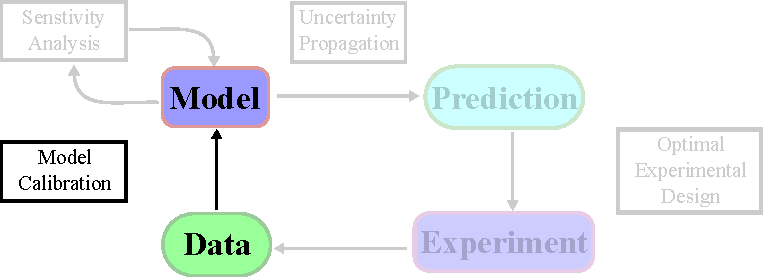
\includegraphics[scale=0.9]{figures/figure-UQcomponetwo-calibration.pdf}
\begin{itemize}
    \item \alert{Sensitivity analysis} identifies the most influential parameters
\end{itemize}
\end{figure}
 }
 
 \only<2>{
 \begin{quote}
   \Large Sensitivity analysis-Determine what are the input parameters whose uncertainty explains the variability of the QoI   
 \end{quote}{}


\begin{columns}
    \column{0.6\textwidth}
    \begin{itemize}
        \item detect input parameters whose uncertainty has \alert{no impact} on the output variability
        \item detect input parameters which allow one to best \alert{decrease the output variability} when set to a deterministic value
        \item detect \alert{interactions} between paramters
    \end{itemize}
    \column{0.4\textwidth}
\begin{figure}          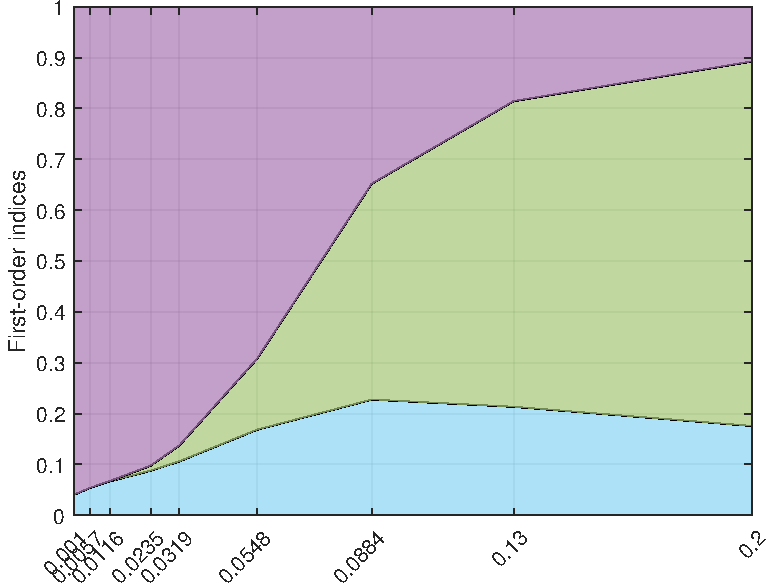
\includegraphics[scale=0.45]{figures/figure-Sobol.pdf}
\end{figure} 
\end{columns}
 }

\only<3>{
\begin{block}{Total variance:}
\begin{equation*}
D\equiv \text{Var}[\mathcal{M}(\boldsymbol{X}) ]
= \text{Var}[\sum_{u \subset \{1,\cdots,M\}} \mathcal{M}_{u}(\boldsymbol{X}_{u}) ]
= \sum_{u \subset \{1,\cdots,M\}} \text{Var}[\mathcal{M}_{u}(\boldsymbol{X}_{u}) ] 
\end{equation*}    
\end{block}

\begin{itemize}
    \item Sobol's indice:
    \begin{equation*}
S_u   \overset{\mathrm{def}}{=} \frac{\text{Var}[\mathcal{M}_{u}(\boldsymbol{X}_{u}) ] }{D} 
    \end{equation*}

    \item First-order Sobol's indice:
     \begin{equation*}
S_i = \frac{D_i}{D} = \frac{\text{Var}[\mathcal{M}_{i}(\boldsymbol{X}_{i}) ] }{D}
    \end{equation*}
    Quantify the effect of each input parameter \alert{separately}

    \item Total Sobol's indice:
    \begin{equation*}
S_{i}^{T} \overset{\mathrm{def}}{=}  
\sum_{u \supset i} S_u
    \end{equation*}
    Quantify the \alert{total effect} of $x_{i}$, including \alert{interactions} with other variables
\end{itemize}
}

 \end{frame}
 %--------------------------------------------------------------------------------------------------
\begin{frame}
 \frametitle{UQ components three-Optimum Experimental design}
 \only<1>{
 \begin{figure} 
 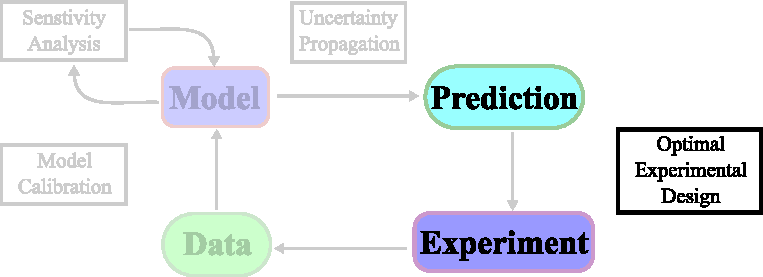
\includegraphics[scale=0.9]{figures/figure-UQcomponent_ActiveLearning.pdf}
\end{figure} 
 }

 \only<2>{

  \begin{figure} 
 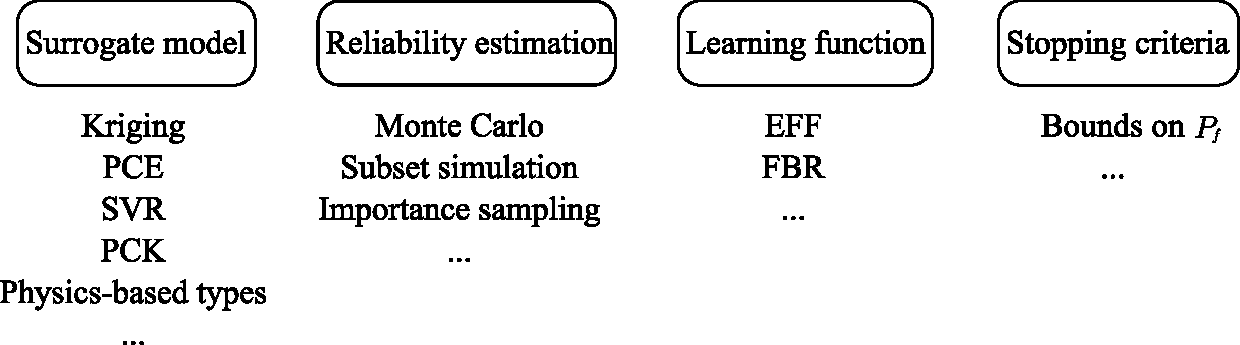
\includegraphics[scale=0.6]{figures/figure-activeLearning_idea.pdf}
\end{figure}
\begin{columns}
    \column{0.5\textwidth}
      \begin{figure} 
 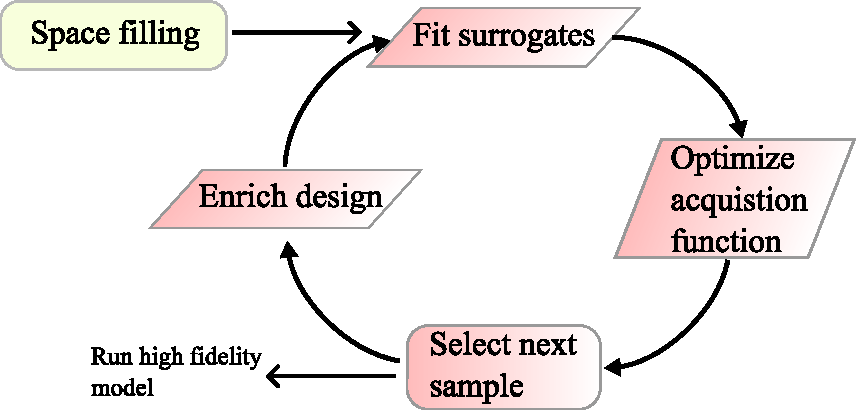
\includegraphics[scale=0.4]{figures/figure-activeLearning_chart.pdf}
\end{figure}
    \column{0.5\textwidth}
    \begin{block}{}
    \begin{itemize}
        \item Not each run is equally important
        \item Save time
    \end{itemize}       
    \end{block}
 
\end{columns}
 }
 \end{frame}
 %--------------------------------------------------------------------------------------------------


 
\begin{frame}
\frametitle{Uncertainty quantification for engineering problems}
Research topics
\begin{itemize}
    \item \textcolor{red}{Uncertainty modelling for engineering systems}
    \item \textcolor{red}{Bayesian model calibration}
    \item Structural reliability analysis
    \item Surrogate models (low dimensions/high dimensions)
    \item Stochastic inverse problem
    \item Global sensitivity analysis
    \item Reliability-based design optimization
    \item ...
\end{itemize}

\end{frame}






\section{\textcolor{orange}{Inverse uncertainty}}
%----------------------------------------------
\subsection{Uncertainty to be considered}

%-----------------------------------------------------------------------------------
\begin{frame}
\frametitle{Choice for UQ inversion}
\begin{columns}
    \column{0.5\textwidth}
        Choice for the UQ method is totally based on the {\textcolor{red}{\textbf{quantity}}} of accessible data:
        \begin{itemize}
            \item  {\textcolor{red}{\textbf{Lack}}} or {\textcolor{red}{\textbf{no}}} data available, model can be solely based on expert judgement
            \item {\textcolor{red}{\textbf{Substantial}}} volume data available, model can fully use statistical inference (e.g., the methods of moments)
            \item {\textcolor{red}{\textbf{Combination}}} of two above: Bayesian methods
            \begin{equation*}           \pi(\boldsymbol{x}|\mathcal{Y}) = \frac{{\mathcal{L}(\boldsymbol{x}|\mathcal{Y}) \cdot \pi(\boldsymbol{x})}}{{\pi(\mathcal{Y})}} 
            \end{equation*}
        \end{itemize}
    
    \column{0.5\textwidth}
        \begin{figure}[!ht]       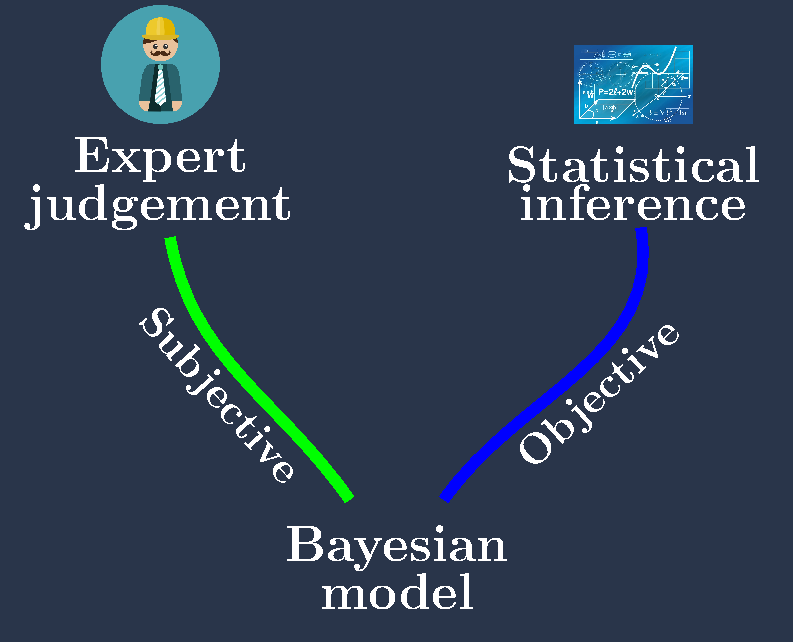
\includegraphics[scale=0.6]{figures/figure_objvssub.pdf}
        \end{figure}
\end{columns}
    
\end{frame}
%===================================================================================================================
\begin{frame}
\frametitle{Posing the probabilistic problem}
\begin{block}{Uncertainties in math form:}
\begin{equation*}
\mathcal{Y}_i = \tilde{\mathcal{M}}(\boldsymbol{x}_i,\boldsymbol{\theta}^{\star}) 
+ \delta(\boldsymbol{x}_i)+
\boldsymbol{\epsilon}_{i}, i=1,\cdots,N
\end{equation*}
$\mathcal{Y}_i$: observation; $\boldsymbol{x}_i$: control inputs; $\boldsymbol{\theta}^{\star}$: true value of calibrated parameters; $\tilde{\mathcal{M}}$: forward model; $\delta$: model discrepancy; $\boldsymbol{\epsilon}_{i}$: observation error  
\end{block}

\begin{block}{Three speficic types of uncertainties (mixed with aleatoric and epistemic): }
\begin{itemize}
    \item observation error
    \item model discrepancy
    \item input space uncertainties
\end{itemize}    
\end{block}

\begin{alertblock}{Should we consider aleatoric uncertainty (irreducible) in the inversion process?}
\begin{itemize}
    \item Or all burden will be shared by other epistemic uncertainty \alert{unreasonably}
\end{itemize}
    
\end{alertblock}
 
\end{frame}







%--------------------------------------------------------------------------------
\subsection{How likelihood dealing with uncertainties?}
\begin{frame}
    

\begin{block}{If only consider a Gaussian type observation error}
\begin{equation*}
\mathcal{Y}_i = \tilde{\mathcal{M}}(\boldsymbol{x}_i,\boldsymbol{\theta}^{\star}) +\boldsymbol{\epsilon}_{i}, i=1,\cdots,N
\end{equation*}
\begin{equation*}        
        \label{eq: Likelihood function}
        \begin{aligned}
         \mathcal{L}(\boldsymbol{\theta}|\mathcal{Y}) =& \prod_{i=1}^{N} N(\mathcal{Y}_{i}|\tilde{\mathcal{M}}(\boldsymbol{x}_i,\boldsymbol{\theta}),\boldsymbol{\Sigma}) \\
         =& \prod_{i=1}^{N}\frac{1}{\sqrt{(2 \pi)^{N_{\rm{out}}}{\rm{det}}         (\boldsymbol{\Sigma})}}\exp\left(-\frac{1}{2}\left(\mathcal{Y}_{i} - \tilde{\mathcal{M}}(\boldsymbol{x}_i,\boldsymbol{\theta})\right)^{\mathsf{T}} \boldsymbol{\Sigma}^{-1}\left(\mathcal{Y}_{i} - \tilde{\mathcal{M}}(\boldsymbol{x}_i,\boldsymbol{\theta})\right)\right) 
        \end{aligned}
        \end{equation*}  
\end{block}

\begin{alertblock}{In real life, only one source of uncertainty is not convincing enough}
\begin{figure}[!ht]       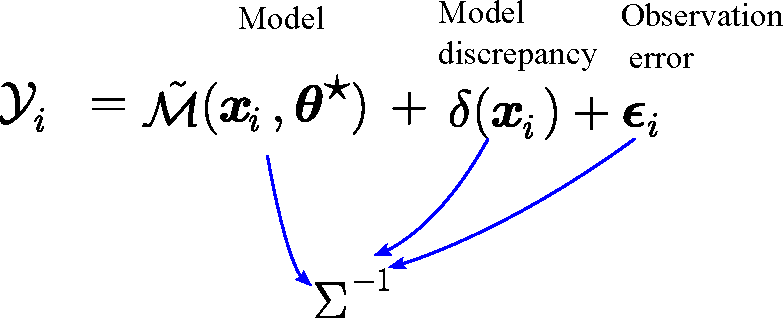
\includegraphics[scale=0.55]{figures/figure-CoVUncertainty.pdf}
\end{figure}
    
\end{alertblock}


\end{frame}
%--------------------------------------------------------------------------------
\begin{frame}
\frametitle{Bayesian inference}
\begin{block}{Difficulty with calculating evidence $\pi(\mathcal{Y})$}
\begin{equation*}               \pi(\boldsymbol{x}|\mathcal{Y}) = 
\frac{{\mathcal{L}(\boldsymbol{x}|\mathcal{Y}) \cdot \pi(\boldsymbol{x})}}{{\pi(\mathcal{Y})}}
= \frac{{\mathcal{L}(\boldsymbol{x}|\mathcal{Y}) \cdot \pi(\boldsymbol{x})}}
{\int_{\mathcal{D}_{\boldsymbol{X}}} 
    \pi(\boldsymbol{x}) \pi(\mathcal{Y}|\boldsymbol{x}) {\rm{d}} \boldsymbol{x}}
\end{equation*}  
\end{block}

Computing evidence ${\pi(\mathcal{Y})}$ is not a tractable problem. A common strategy is using \textit{conjugate priors}  
\begin{itemize}
    \item static Bayesian network
    \item variant elimintion/ belief propagation
    \item kalman filtering
\end{itemize}

\begin{block}{Computational methods:}
 \begin{equation*}               \pi(\boldsymbol{x}|\mathcal{Y}) \approx 
{\mathcal{L}(\boldsymbol{x}|\mathcal{Y}) \cdot \pi(\boldsymbol{x})}
\end{equation*}     
\end{block}
Samples from the posterior can be obtained through \textit{Sampling methods} or \textit{Optimization methods}
\end{frame}
%-------------------------------------------------------------------------------------------
\subsection{Sampling methods}
\begin{frame}
\only<1>{
\begin{definition}
\textbf{Optimisation based approximation}: This method usually refers to variational inference. The basic principle is adopting some analytical distributions to approximate the posterior based on some loss functions
\end{definition}

\begin{block}{PROS and CONS:}
 \begin{itemize}
     \item[\scalebox{1.5} {\color{green}\checkmark}] computational efficient and work well with large model
     \item[\scalebox{1.5} {\color{green}\checkmark}] has absolute converging criteria which makes easy t odetermine when to stop
     \item[\scalebox{1.5}{\color{red}$\times$}] unlikely to discover the globally optimal solution
     \item[\scalebox{1.5}{\color{red}$\times$}] precision constrained by the structure of approximaiton
     
 \end{itemize}   
\end{block}
}


\only<2>{
\begin{definition}
\textbf{Monte Carlo sampling}: These techniques produce random samples from a proposal distribution, utilizing
them to estimate both the posterior distribution and the associated statistics
\end{definition}

Some are:
\begin{itemize}
    \item probability density tranform
    \item rejection sampling
    \item importance sampling
    \item sequential Monte Carlo (e.g., particle filtering)
    \item Markov Chain Monte Carlo (MH, HMC, AIES)
\end{itemize}

}

    
\end{frame}



%------------------------------------------------------------------------------------
\begin{frame}
\frametitle{SMC vs MCMC}
\only<1>{
\begin{quote}
    ... non-iterative methods for generating independent
samples..., we discuss an iterative method known as Markov Chain Monte
Carlo, or \alert{MCMC} for short, which produces dependent samples but \alert{which works well in high
dimensions}...\footfullcite{murphy2012}
\end{quote}


}

\only<2>{

\begin{columns}
    \column{0.45\textwidth}
    \begin{block}{SMC} \animategraphics[autoplay,loop,width=\textwidth]{1}{figures-gif/PF/particlefilter-}{0}{12}        
    \end{block}
    Source:\hyperlink{https://medium.com/@mathiasmantelli/particle-filter-part-3-motion-and-measurement-models-be79857a5490}{weblink}
    \column{0.45\textwidth}
     \begin{block}{MCMC} \animategraphics[autoplay,loop,width=\textwidth]{1}{figures-gif/MCMC/MCMC-}{1}{26}        
    \end{block} 
    Source:\hyperlink{https://www.cdslab.org/DSP2019F/announcement/0-student-professor-connection-day}{weblink}
\end{columns}

}

\end{frame}


\section{\textcolor{black}{Final goal of UQ}}
\begin{frame}
\frametitle{A unified and scable digital twin}
Digital twin is used to:

\begin{itemize}
        \item  Visualize the calibration and prediction
    \item Make prompt actions      
\end{itemize}
\pause

\begin{figure} 
\only<2>{
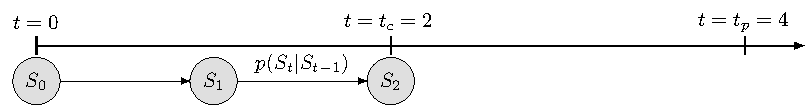
\includegraphics[scale=0.75]{figures/figure-POMDP1.pdf}
}
\only<3>{
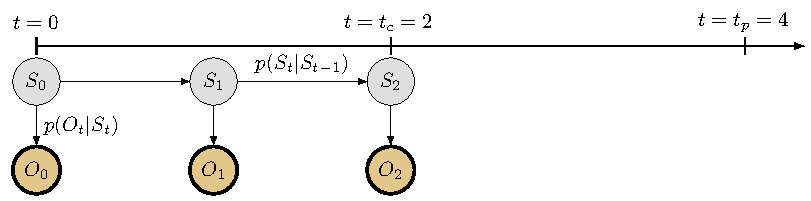
\includegraphics[scale=0.8]{figures/figure-POMDP2.pdf}
}
\only<4>{
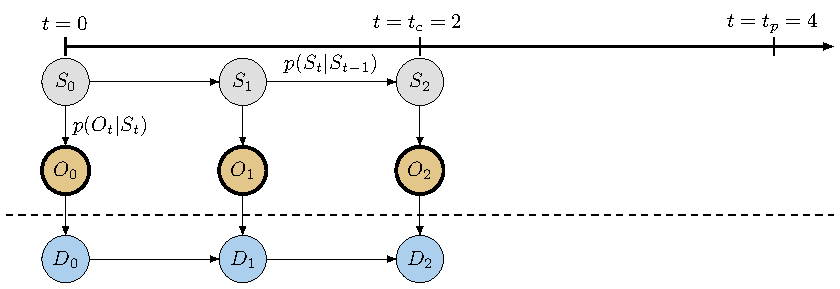
\includegraphics[scale=0.8]{figures/figure-POMDP3.pdf}
}
\only<5>{
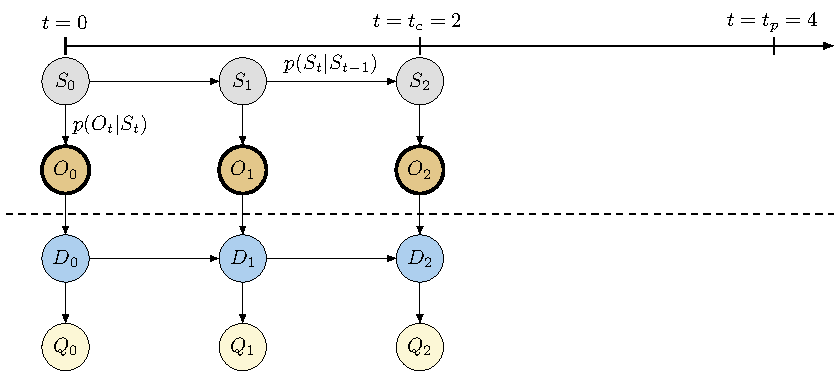
\includegraphics[scale=0.8]{figures/figure-POMDP4.pdf}
}
\only<6>{
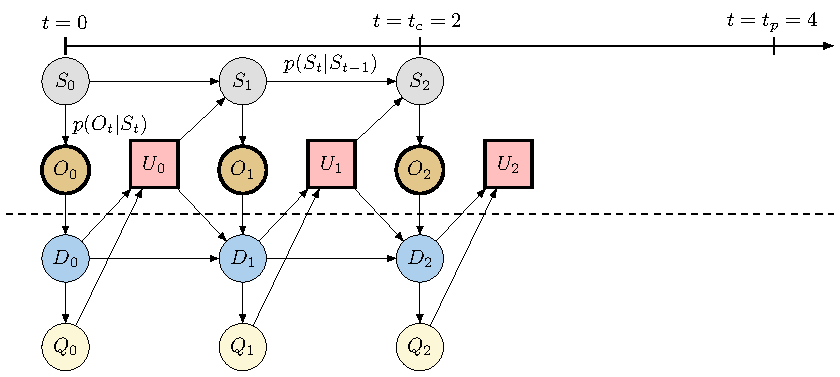
\includegraphics[scale=0.8]{figures/figure-POMDP5.pdf}
}
\only<7>{
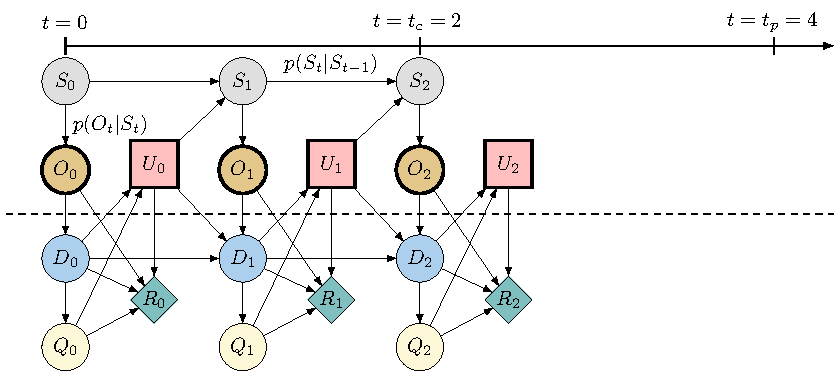
\includegraphics[scale=0.8]{figures/figure-POMDP6.pdf}
}
\only<8>{
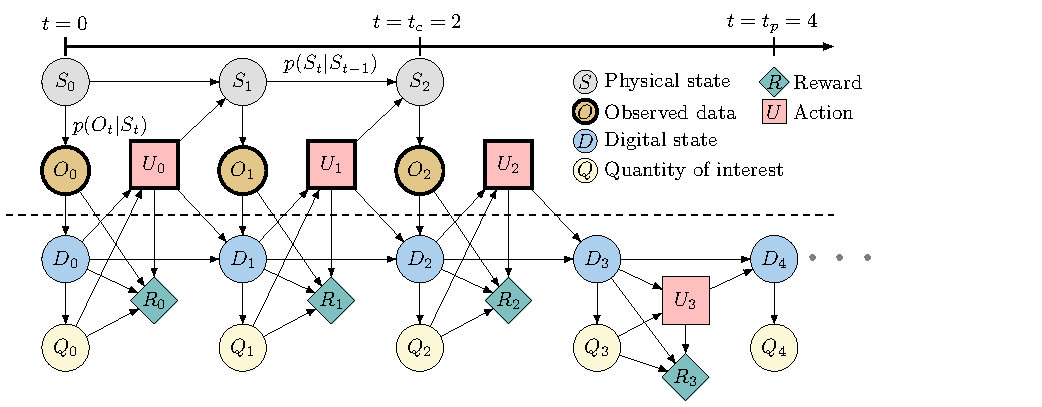
\includegraphics[scale=0.8]{figures/figure-POMDP7.pdf}
}
\end{figure}
 
\end{frame}








\section{\textcolor{black}{Summary}}
\begin{frame}

\frametitle{Summary}

\begin{enumerate}
\setlength\itemsep{1em}
    \item In engineering, we should notice which uncertainty is \alert{aleatoric} or \alert{epistemic} or \alert{mixed type}
 
    \item Four UQ components are \alert{equally} important

    \item Consider different types of uncertainty into Bayesian inference required \alert{linked with likelihood}

    \item \alert{Digital twin}-final goal of UQ in geotechnics 
\end{enumerate}

    
\end{frame}






%-----------------------------------------------------
%---------------References
\begin{frame}[allowframebreaks]% Use [allowframebreaks] to allow automatic splitting across slides if the content is too long
	\frametitle{References}
\printbibliography
\end{frame}


%	CLOSING SLIDE
%----------------------------------------------------------------------------------------

\begin{frame}[plain] % The optional argument 'plain' hides the headline and footline
	\begin{center}
		{\Huge Thank you!}
		
		\bigskip\bigskip % Vertical whitespace
		
		{\LARGE Questions? Comments?}
	\end{center}
\end{frame}

%----------------------------------------------------------------------------------------



%=========================================
%=============appendix===================
%%%%----------------------------------------------------------------------------------------+
\backupbegin
% And your backup slides here

\begin{frame}
\frametitle{Appendix:}
\framesubtitle{Aleatoric to epistemic}
\begin{figure}[!ht]       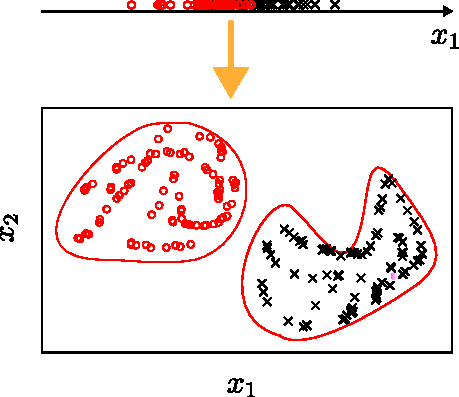
\includegraphics[scale=1]{figures/figure-transform.pdf}
\end{figure}
    
\end{frame}
%%%%----------------------------------------------------------------------------------------
\begin{frame}
\frametitle{Appendix:}
\framesubtitle{Sequential Bayesian inference}
\begin{figure}[!ht]       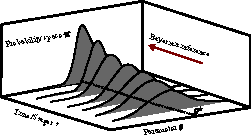
\includegraphics[scale=2.55]{figures/figure-SBI.pdf}
\end{figure}
    
\end{frame}


%=====================================================

%================================================
\begin{frame}
\frametitle{Appendix:}
\framesubtitle{Inverse probability transform}
\begin{itemize}
    \item Inverse probability transform
\end{itemize}
\begin{figure}[ht]
    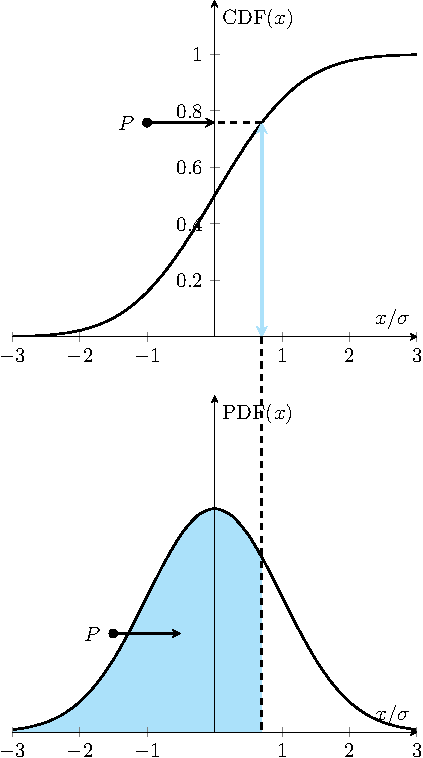
\includegraphics[width = 35mm]{figures/figure-CDF.pdf}
\end{figure}
\end{frame}
%================================================

\begin{frame}
\frametitle{Appendix:}
\framesubtitle{Rejection sampling}
\begin{itemize}
    \item Rejection sampling
\end{itemize}
\begin{figure}[ht]
    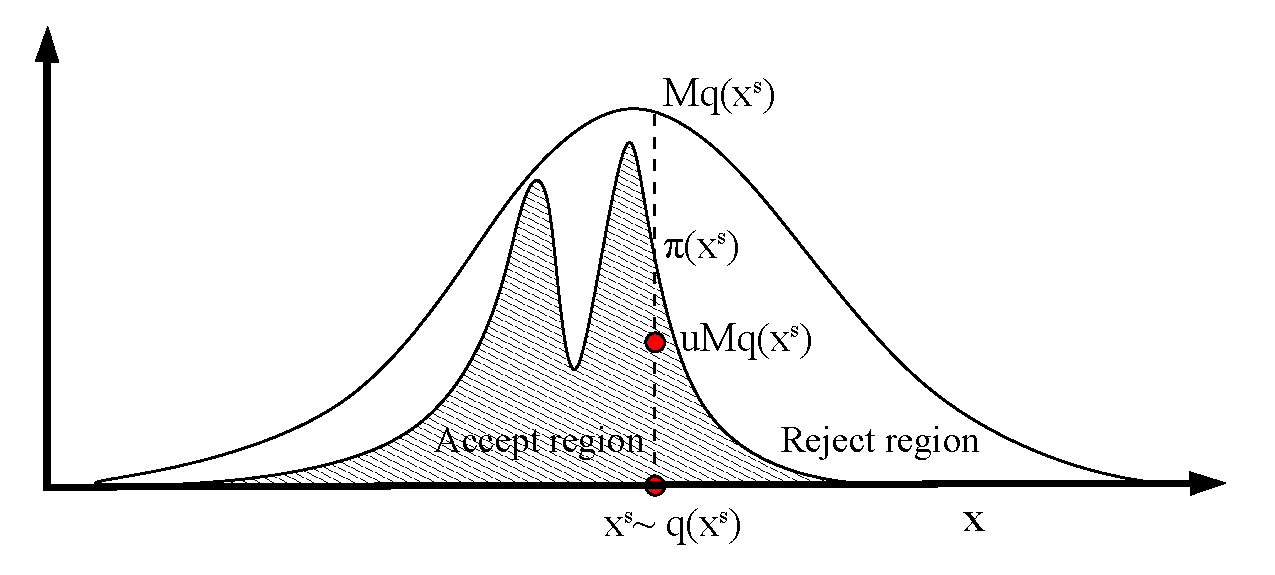
\includegraphics[width = 110mm]{figures/figure-rejectionsampling.pdf}
\end{figure}
\end{frame}
%================================================

\begin{frame}
\frametitle{Appendix:}
\framesubtitle{importance sampling}
\begin{equation*}
E[f(\boldsymbol{x}_{t})] = \int f(\boldsymbol{x}_{t})\pi(\boldsymbol{x}_{t}) d\boldsymbol{x}_{t}
\approx \frac{1}{S}\sum_{s=1}^{S} f(\boldsymbol{x}_{t}^{s})
\end{equation*}


\begin{equation*}
    E[f(\boldsymbol{x}_{t})] = \int f(\boldsymbol{x}_{t})\pi(\boldsymbol{x}_{t}) d\boldsymbol{x}_{t} = \int f(\boldsymbol{x}_{t})\frac{\pi(\boldsymbol{x}_{t})}{q(\boldsymbol{x}_{t})}q(\boldsymbol{x}_{t}) d\boldsymbol{x}_{t}
    \approx \frac{1}{S} \sum_{s=1}^{S} f(\boldsymbol{x}_{t}^{s})\frac{\pi(\boldsymbol{x}_{t}^{s})}{q(\boldsymbol{x}_{t}^{s})}
\end{equation*}

    \begin{itemize}
        \item Require a proper proposal distribution $q(\boldsymbol{x}_{t})$

    \end{itemize}

\end{frame}
%=======================================================
\begin{frame}
\frametitle{Appendix:}
\framesubtitle{Metropolish-Hasting}
\begin{equation*}
f(\boldsymbol{x}_{t}^{s+1}|\boldsymbol{x}_{t}^{s})=\rm{min}(1,\alpha)
\end{equation*}
\begin{equation*}
\alpha = {\rm{min}} (1,
\frac{q(\boldsymbol{x}_{t}^{s}|\boldsymbol{x}_{t}^{s+1})  \pi(\boldsymbol{x}_{t}^{s+1}|\mathcal{Y}_{t})}
{q(\boldsymbol{x}_{t}^{s+1}|\boldsymbol{x}_{t}^{s})   \pi(\boldsymbol{x}_{t}^{s}|\mathcal{Y}_{t})} )
\end{equation*}

\end{frame}
%============================================================
\begin{frame}
\frametitle{Appendix:}
\framesubtitle{Metropolish-Hasting}
\begin{algorithm}[H]
    \caption{MH algorithm at $t_{th}$ step}
    \label{Algorithm:MH}
    \KwData{ $q(\boldsymbol{x}_{t})$: Proposal distribution; $\pi(\boldsymbol{x}_{t}|\mathcal{Y})$: Target posterior.}
    \KwResult{MCMC samples at $t_{th}$ stage: $\mathcal{X}_{t} = \{\boldsymbol{x}_{t}^{1},\cdots,\boldsymbol{x}_{t}^{N_{\mathcal{X}}}\}$}
    Initialization $\boldsymbol{x}_{t}^{1} \in \mathcal{D}_{\bm{X}}$\; 
    \For{$s \gets 2 \ to  \ N_{\mathcal{X}}$}{
        Sample $\boldsymbol{x}_{t}^{s+1} \sim q(\boldsymbol{x}_{t}^{s+1}|\boldsymbol{x}_{t}^{s})$;\\
        Compute acceptance probability $\alpha$;\\
        Compute $f\left(\boldsymbol{x}_{t}^{s+1}|\boldsymbol{x}_{t}^s\right)=\min{\left(1,\alpha\right)}$;\\
        Sample $u \sim \mathcal{U}\left(0,1\right)$;\\
        Set candidate sample $\boldsymbol{x}_{t}^{(\star)}$ to $\boldsymbol{x}_{t}^{s+1}$ with probability $\alpha$;} 
\end{algorithm}
\end{frame}
%======================================================================================
\begin{frame}
\frametitle{Appendix:}
\framesubtitle{Metropolish-Hasting}
\begin{figure}[ht]
    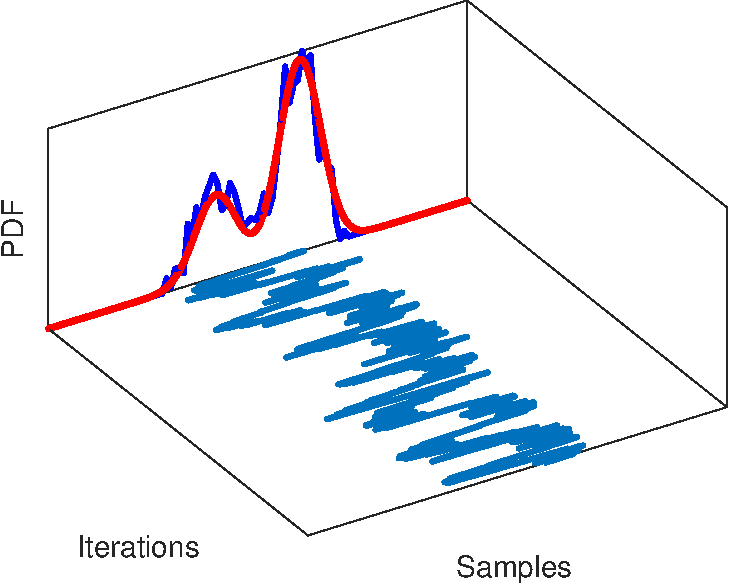
\includegraphics[width = 80mm]{figures/figure-MCMC_sampling.pdf}
\end{figure}
\end{frame}


%=============================================================================
\begin{frame}
\frametitle{Appendix:}
\framesubtitle{AIES}
\begin{equation*}
\boldsymbol{x}_{t}^{(\star)}
=
\boldsymbol{x}_{t\_i}^{(s)}
+
z \cdot 
(\boldsymbol{x}_{t\_j}^{(\tilde{s})} - \boldsymbol{x}_{t\_i}^{(s)})
\end{equation*}
\begin{equation*}
    p(z|a)= \left\{\begin{matrix}
  \frac{1}{\sqrt{z} (2\sqrt{a} - \frac{2}{\sqrt{a} } )}  & {\rm{if} }\ z \in [1 / a, a]  \\
  0 & {\rm{otherwise} }
\end{matrix}\right.
\end{equation*}
\begin{equation*}
    \alpha = {\rm{min}}
(1,
z^{M-1} 
\frac{\pi({x}_{t}^{(\star)}|\mathcal{Y})}
{\pi({x}_{t\_{i}}^{(s)}|\mathcal{Y})} 
)
\end{equation*}
\end{frame}

%=========================================================
\begin{frame}
\frametitle{Appendix:}
\framesubtitle{AIES}
\begin{algorithm}[H]    
    \caption{AIES algorithm at $t_{th}$ step}
    \label{Algorithm:AIES}
    \KwData{$\pi(\boldsymbol{x}_{t}|\mathcal{Y})$: Target posterior; tuning parameter $a$}
    \KwResult{MCMC samples at $t_{th}$ stage: $\mathcal{X}_{t} = \{ \mathcal{X}_{t\_1},\cdots,\mathcal{X}_{t\_N_{chain}}\}$), with $\mathcal{X}_{t\_i}=\{ \boldsymbol{x}_{t\_i}^{1},\cdots,\boldsymbol{x}_{t\_i}^{N_{\mathcal{X}}}\}$}
    Initialization $N_{chain}$ samples $\{  \boldsymbol{x}_{t\_1}^{1},\cdots,\boldsymbol{x}_{t\_{N_{chain}}}^{1}\}$, with $\boldsymbol{x}_{t\_i}^{1} \in \mathcal{D}_{\boldsymbol{X}}$\
    
    \For{$s \gets 2 \ to  \ N_{\mathcal{X}}$}{
        \For{$ i \in \{ 1,\cdots,N_{chain}\}$}{
            Pick random $j$ from $\{ 1,\cdots,N_{chain}\} \backslash i$;\\
            Propose ${x}_{t}^{(\star)}$ with \cref{eq: AIES walker};\\
            Set $\boldsymbol{x}_{t\_i}^{s} = {x}_{t}^{(\star)}$ with probability $\alpha$ (see \cref{eq: AIES acceptance probability});
        }        
        } 
\end{algorithm}
\end{frame}
%=====================================================================================
\begin{frame}
\frametitle{Appendix:}
\framesubtitle{Sequential Monte Carlo}
\begin{equation*}
\label{eq: Bayesian filtering}
\begin{aligned}
   & \boldsymbol{{x}_{t}}  =g(\boldsymbol{{x}_{t-1}}) + \boldsymbol{v} \ \   \ &\rm{(state  \ equation)}\\    
     &\mathcal{Y}_{t}=m(\boldsymbol{{x}_{t}}) + \boldsymbol{w} \ \ \ \ \ &\rm{(observation \  equation)}
\end{aligned}
\end{equation*}

\begin{equation*}
\pi(\boldsymbol{x}_{1:t}|\mathcal{Y}_{1:t})
\approx 
\sum_{s=1}^{S} 
\tilde{w}_{t}^{s}
\delta_{\boldsymbol{x}_{1:t}^{s}}(\boldsymbol{x}_{1:t})
\end{equation*}

\begin{equation*}
\tilde{w}_t^s=\frac{w_t^s}{\sum_{s=1}^{S}{(w_t^s)}}
\end{equation*}

\begin{equation*}
\pi(\boldsymbol{x}_{1:t}|\mathcal{Y}_{1:t})
    \propto 
    \pi(\mathcal{Y}_{t}|\boldsymbol{x}_{t})
    \pi(\boldsymbol{x}_{t}|\boldsymbol{x}_{t-1})
    \pi(\boldsymbol{x}_{t-1}|\mathcal{Y}_{t-1})
\end{equation*}
\end{frame}

%======================================================
\begin{frame}
\frametitle{Appendix:}
\framesubtitle{Sequential Monte Carlo}
\begin{figure}[ht]
    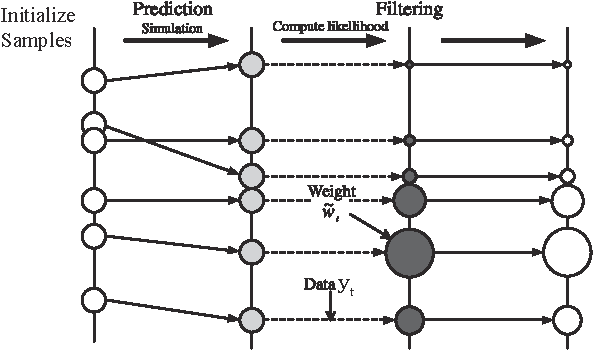
\includegraphics[width = 110mm]{figures/figure-PF-SIS.pdf}
\end{figure}
\end{frame}
%===================================================
\begin{frame}
\frametitle{Appendix:}
\framesubtitle{Sequential Monte Carlo with resampling}
\begin{algorithm}[H]    
    \caption{SISR algorithm at $t_{th}$ step}
    \label{Algorithm:SISR}
    \KwData{Samples $\boldsymbol{x}_{t-1}^{s}$ with weights $w_{t-1}^{s},\ s = \{1,\cdots,N\}$; observation $\mathcal{Y}_{t}$ at $t_{th}$ stage}
    \KwResult{SMC samples with normalized weights $\tilde{w}_{t}^{s}$ at $t_{th}$ stage: $\boldsymbol{x}_{t}^{(\star)} = \{\boldsymbol{x}_{t}^{1},\cdots,\boldsymbol{x}_{t}^{N} \}$)}
    \For{$s \gets 1 \ to  \ N$}{
            Sample from proposal distribution $\boldsymbol{x}_{t}^{s} \sim q(\boldsymbol{x}_{t}^{s}|\boldsymbol{x}_{t-1}^{s},\mathcal{Y}_{t})$;\\
            Compute weight using \cref{eq: PF-modified_weight};
        } 
        Normalized weights;\\
        Calculate degeneracy measure using \cref{eq: SISR_Seff};\\
        \If{$\hat{S}_{eff} < S$}{
        Resample;\\        
        }
\end{algorithm}
\end{frame}
%=====================================================================
\begin{frame}
\frametitle{Appendix:}
\framesubtitle{Sequential Monte Carlo with resampling}
\begin{figure}[ht]
    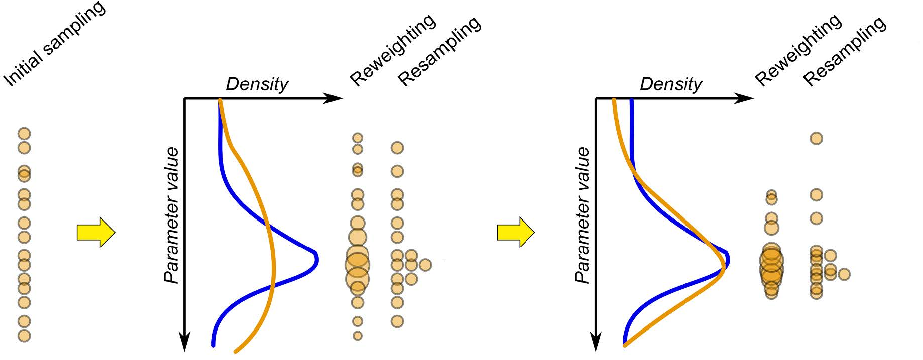
\includegraphics[width = 130mm]{figures/figure-PF-SISR.pdf}
\end{figure}
\end{frame}

%======================================================
\begin{frame}
\frametitle{Appendix:}
\framesubtitle{Visualized PCE}
\begin{figure}[ht]
    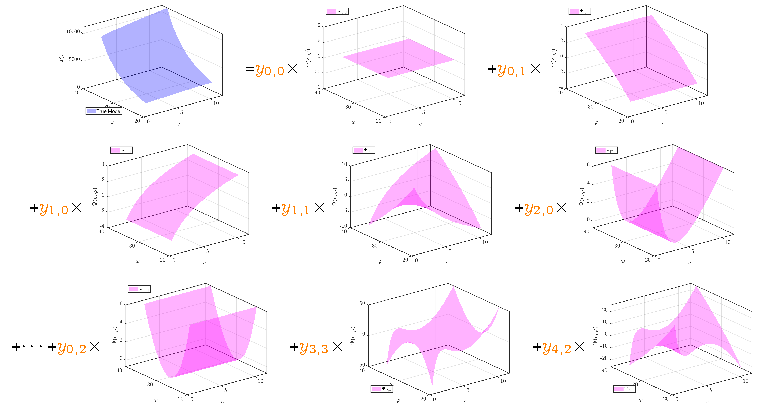
\includegraphics[width = 130mm]{figures/figure-PCE_visualize.pdf}
\end{figure}
\end{frame}
\backupend






\end{document} 